\clearpage
\section{\textsc{Auswertung}}
\subsection{Vermessung der Signale am Oszilloskop}
Die erste Aufgabe war, die Signale des Verstärkers und des Szintillators mit dem Oszilloskop aufzunehmen. Die Zeichnungen, welche wir zu den Signalen anfertigten, finden sich im Anhang. Für das Signal des Vorverstärkers erhielten wir wie erwartet einen sehr steilen, fast senkrechten Anstieg, gefolgt von einer langen Abfalldauer. Für den unipolaren Ausgang des Hauptverstärkers erhielten wir einen positiven Peak. Als Anstiegszeit konnten wir $0,8 \mu s$, als Abfallzeit $1,5 \mu s$ bestimmen. Das Signal hatte eine Amplitude von etwa $7,8 V$. \\
Für den bipolaren Ausgang des Hauptverstärkers konnte - wie es auch der Fall sein sollte - ein positiver Peak, gefolgt von einem negativen Peak beobachtet werden. Wir vermaßen dabei die Anstiegs- und die Abfallzeit nicht, da nur der Nulldurchgang des Signals von Bedeutung ist.\\
\subsection{Spektren von $^{57}Co$ und $^{241}Am$}
Um eine Energiekalibrierung für den Multi Channel Analyzer (MCA) durchführen zu können, nahmen wir für die oben genannten Stoffe ein Energiespektrum auf, um dann die bekannten Energien der Peaks bestimmten Kanälen zuordnen zu können. Da  wir zwei Szintillatoren zur Verfügung stehen hatten, sowie zwei Ausrichtungen der Probe möglich waren, nahmen wir für $^{57}Co$ zunächst für jede Kombination von Ausrichtung und Szintillator ein Energiespektrum auf:\\
\begin{figure}[h] 
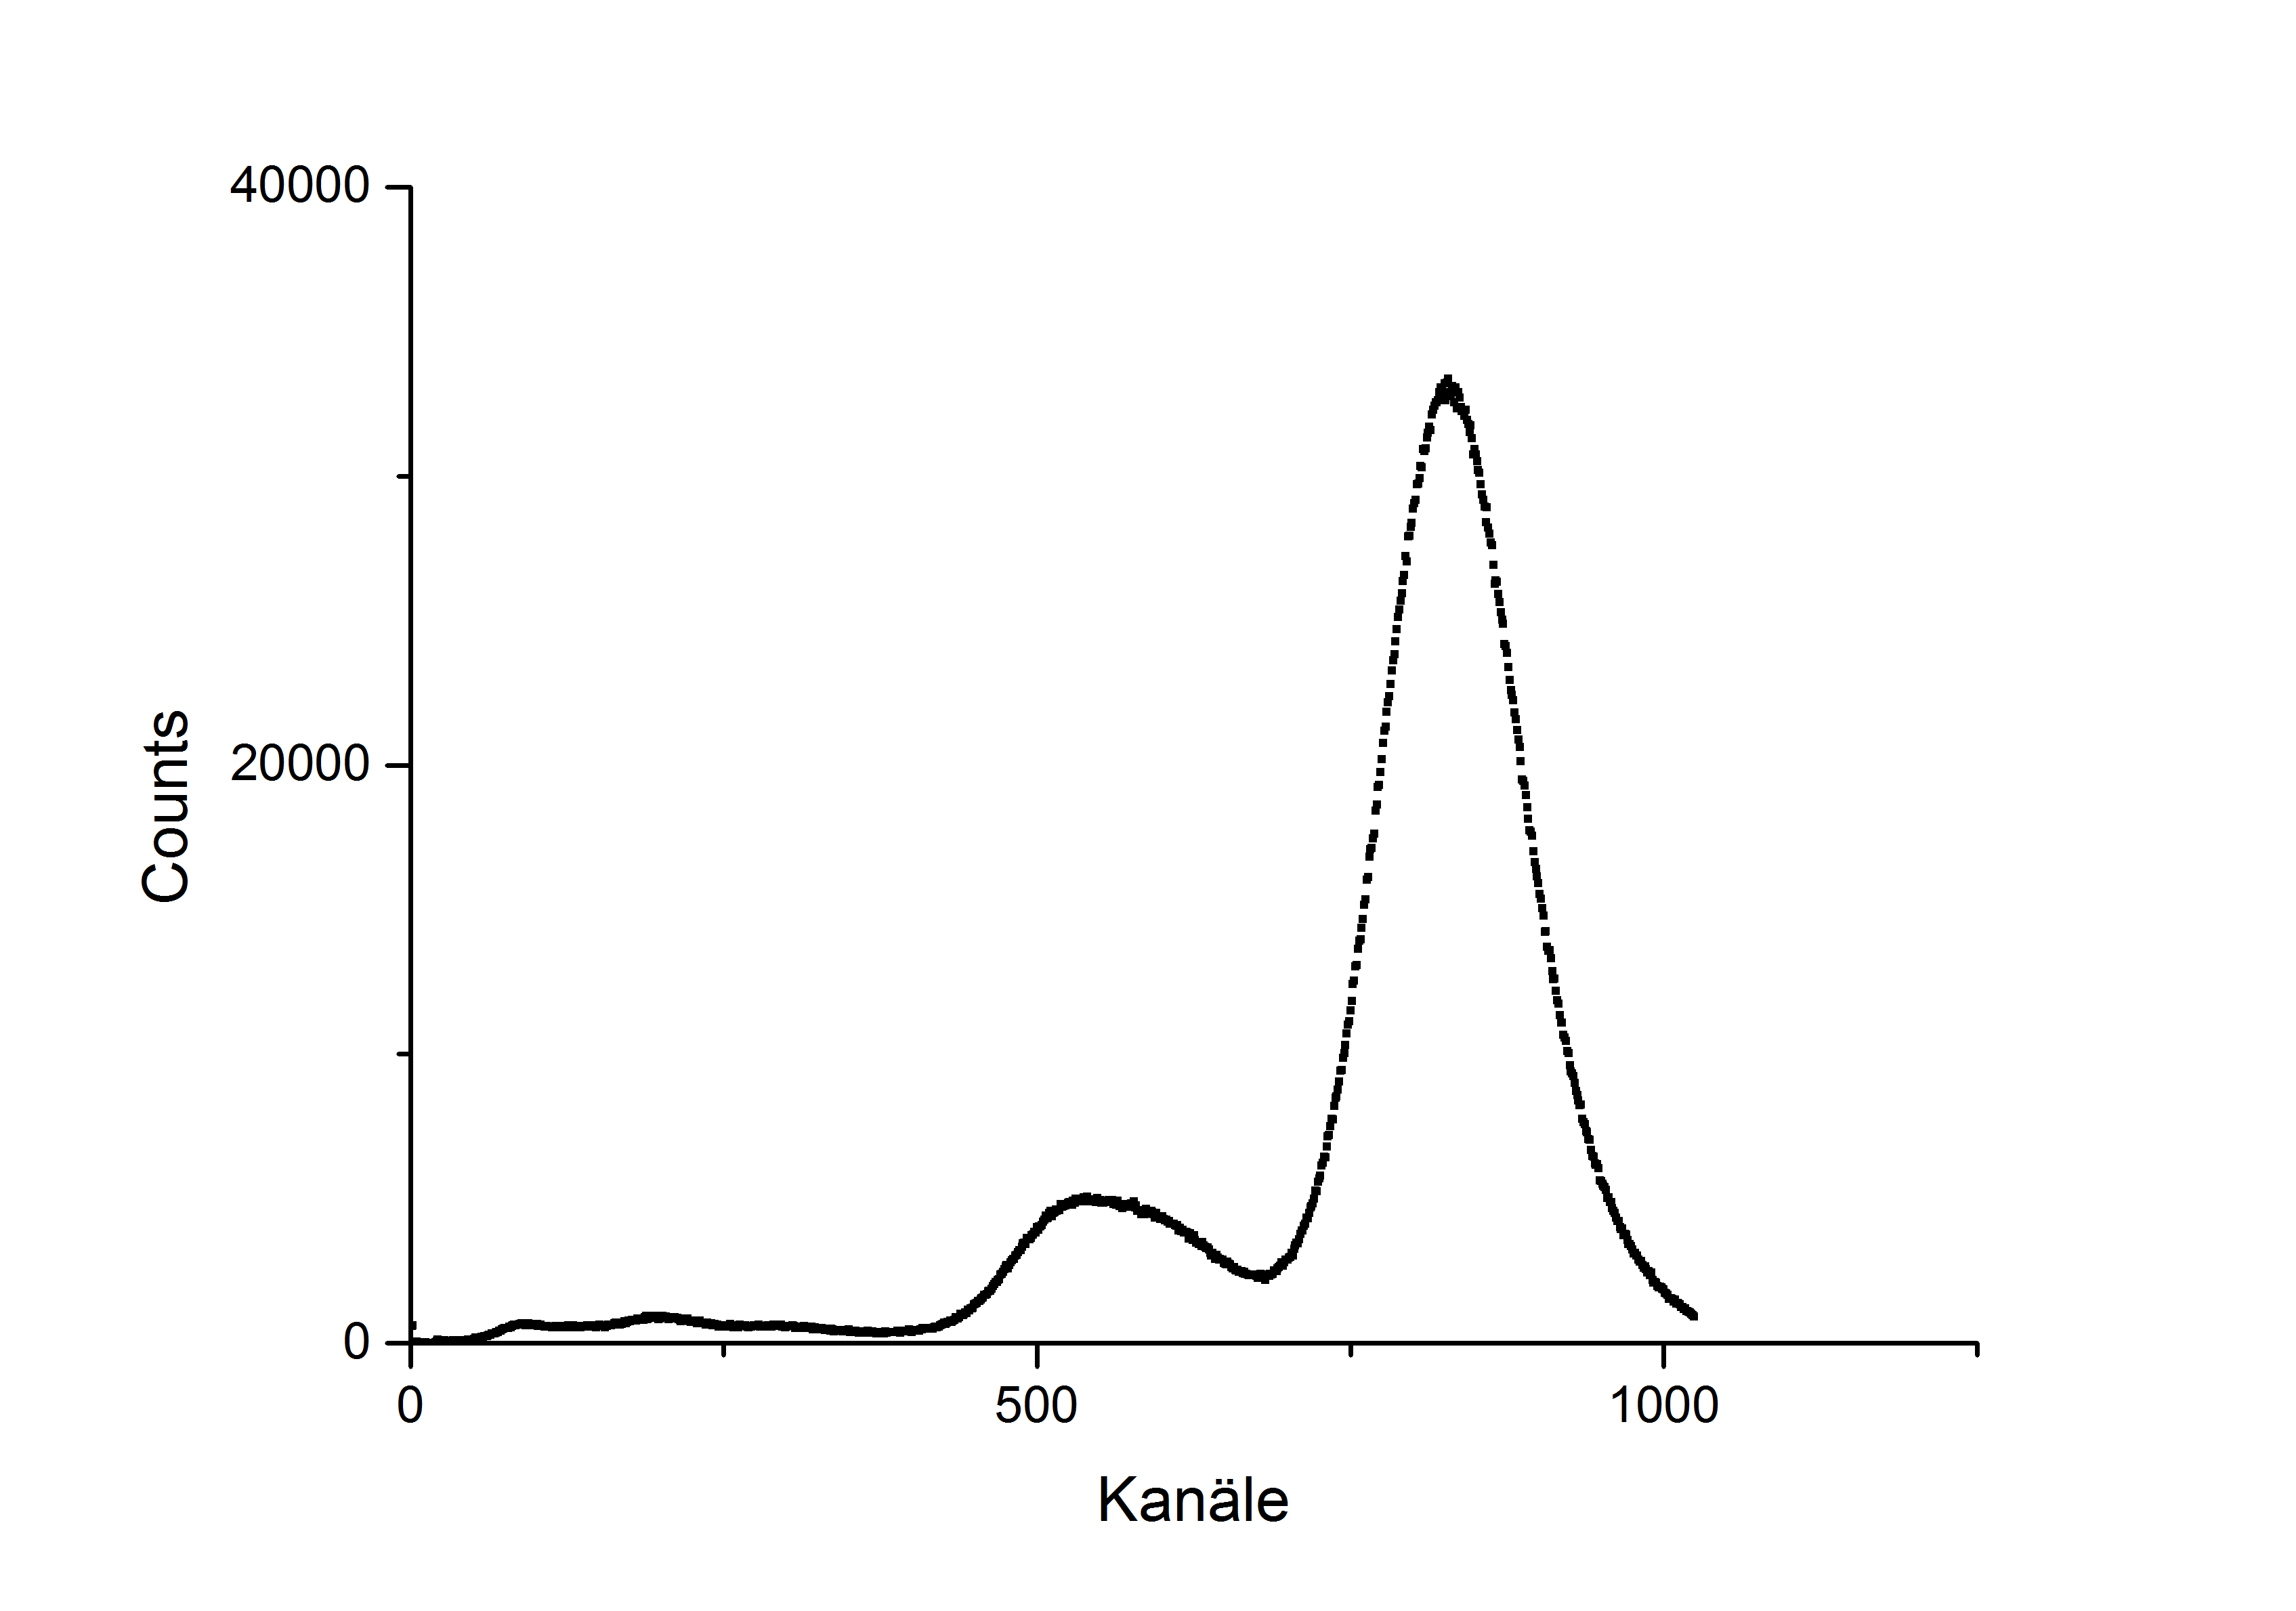
\includegraphics[scale=0.5]{coliszli}
\caption{Szintillator links, Öffnung $^{57}Co$ links}
\end{figure} \\
\begin{figure}[h]
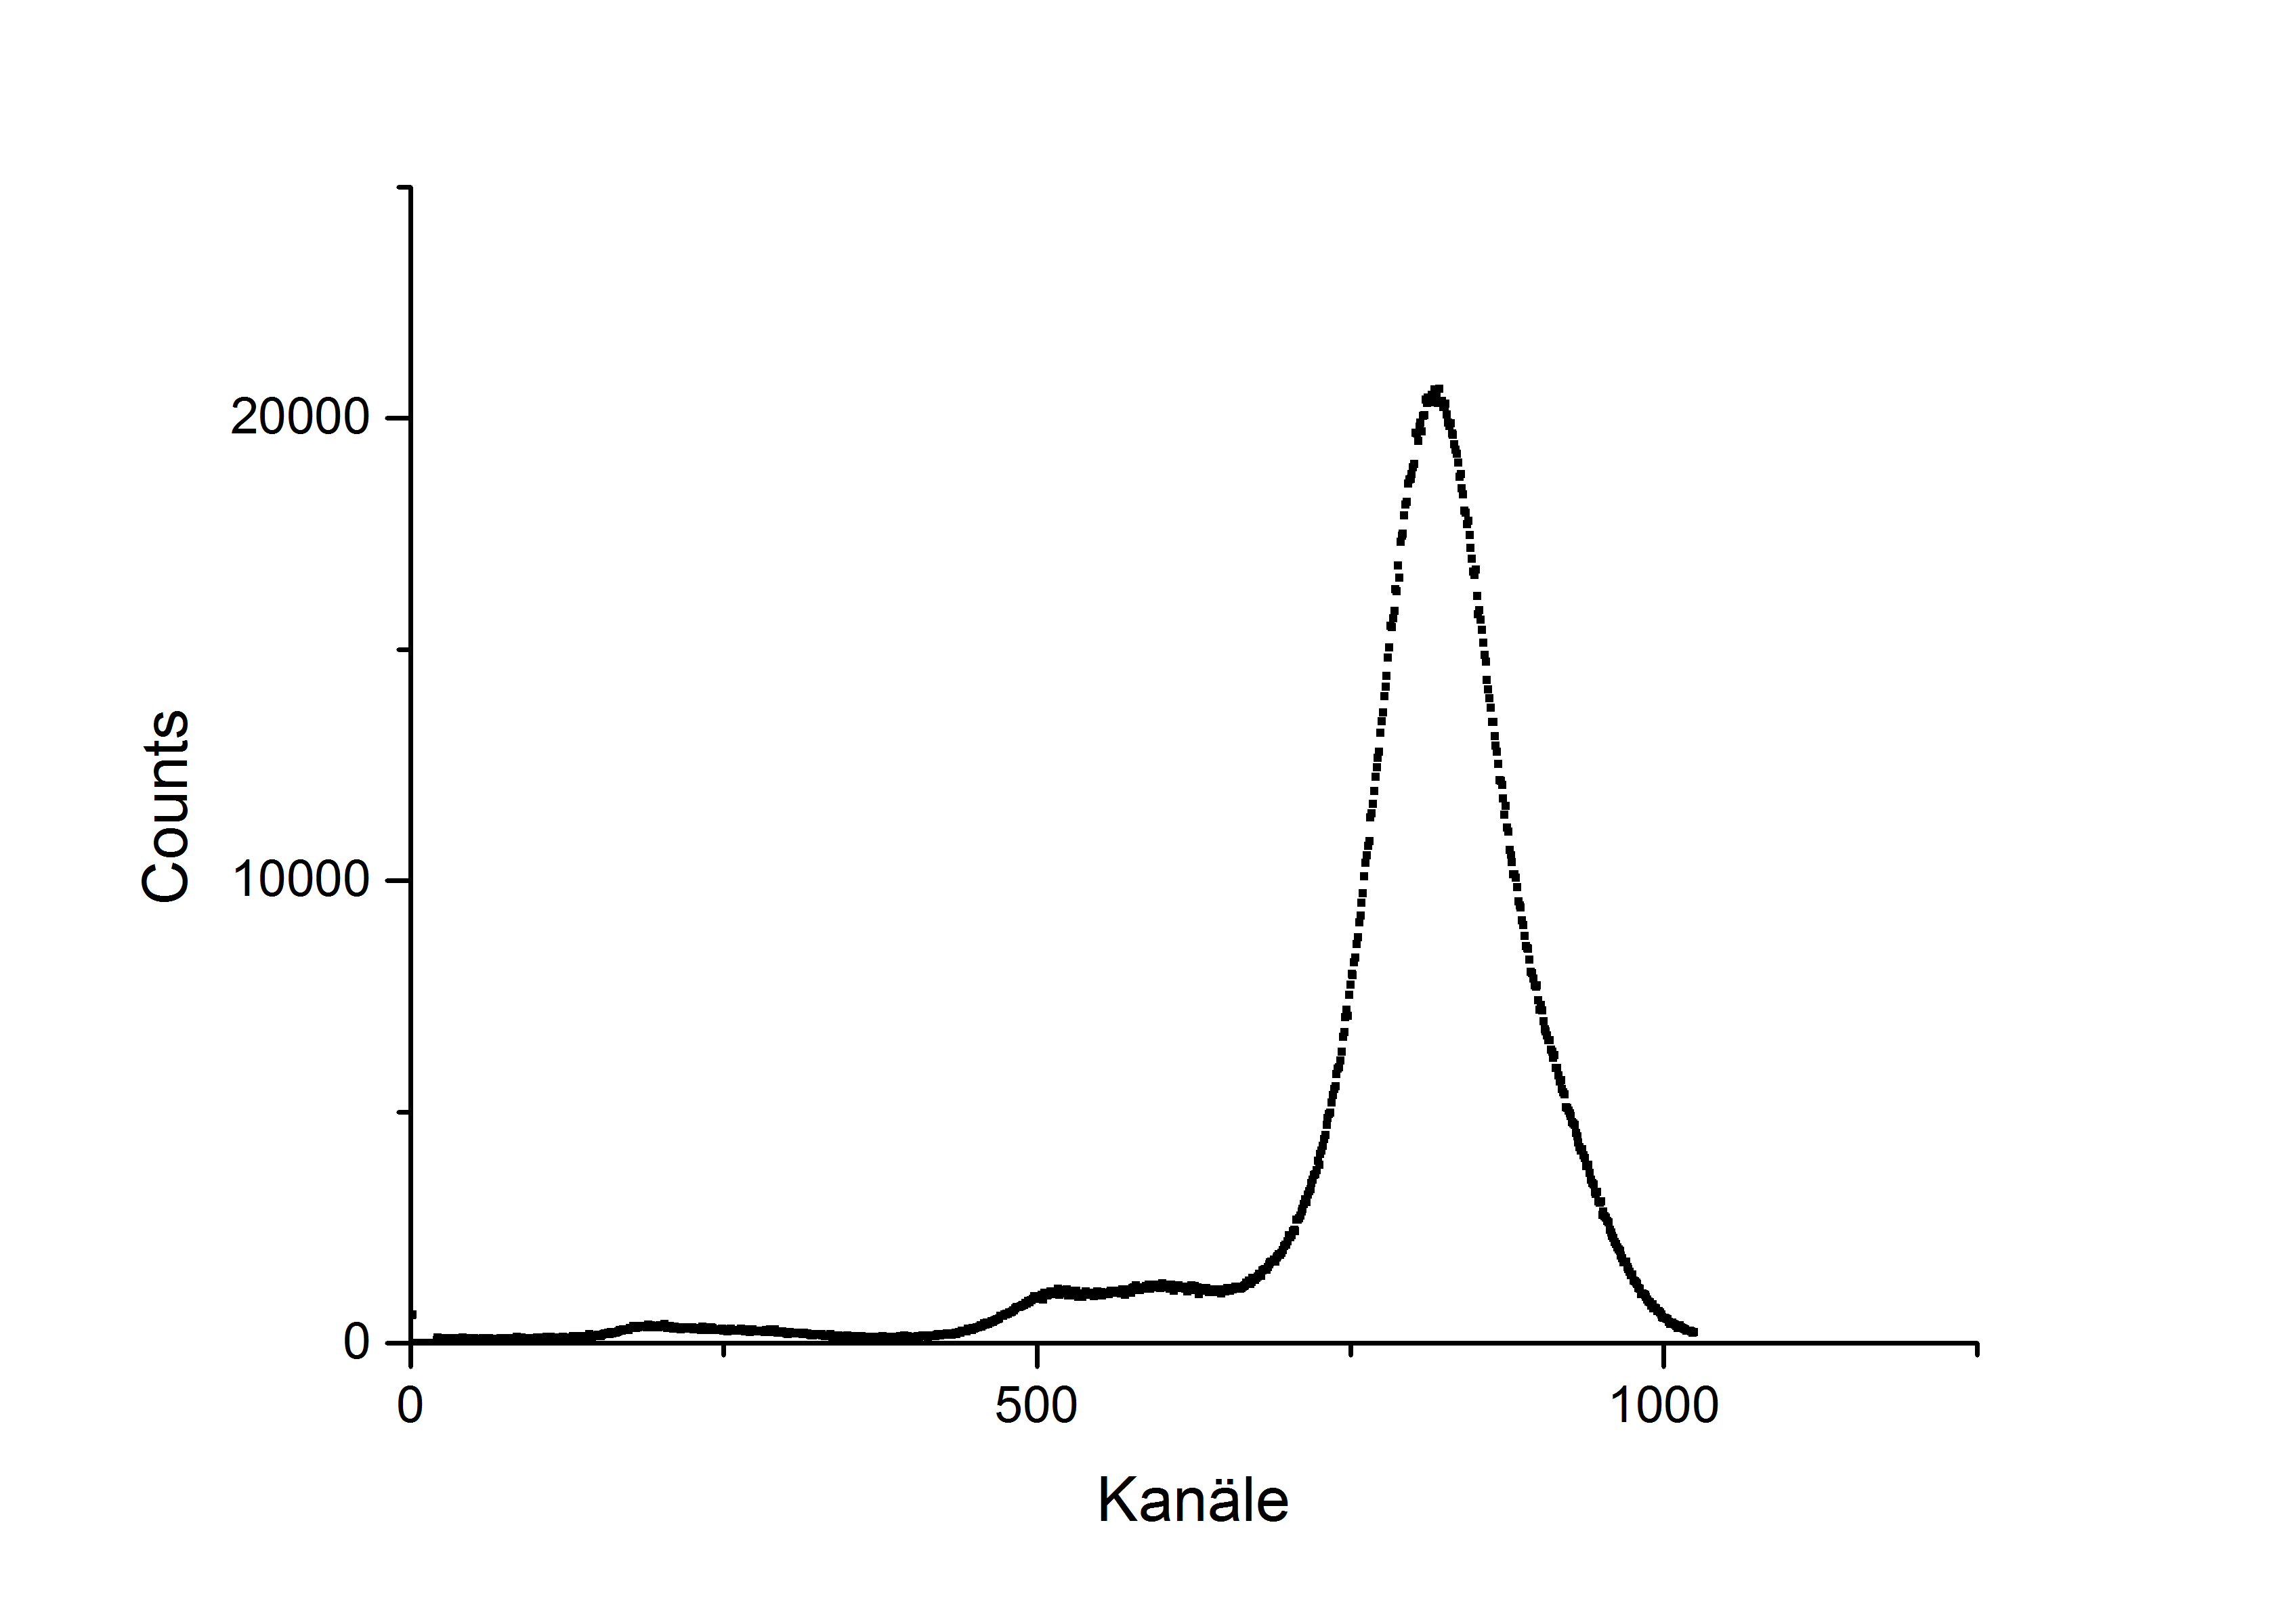
\includegraphics[scale=0.5]{coliszre}
\caption{Szintillator rechts, Öffnung $^{57}Co$ links}
\end{figure}
\begin{figure}[h]
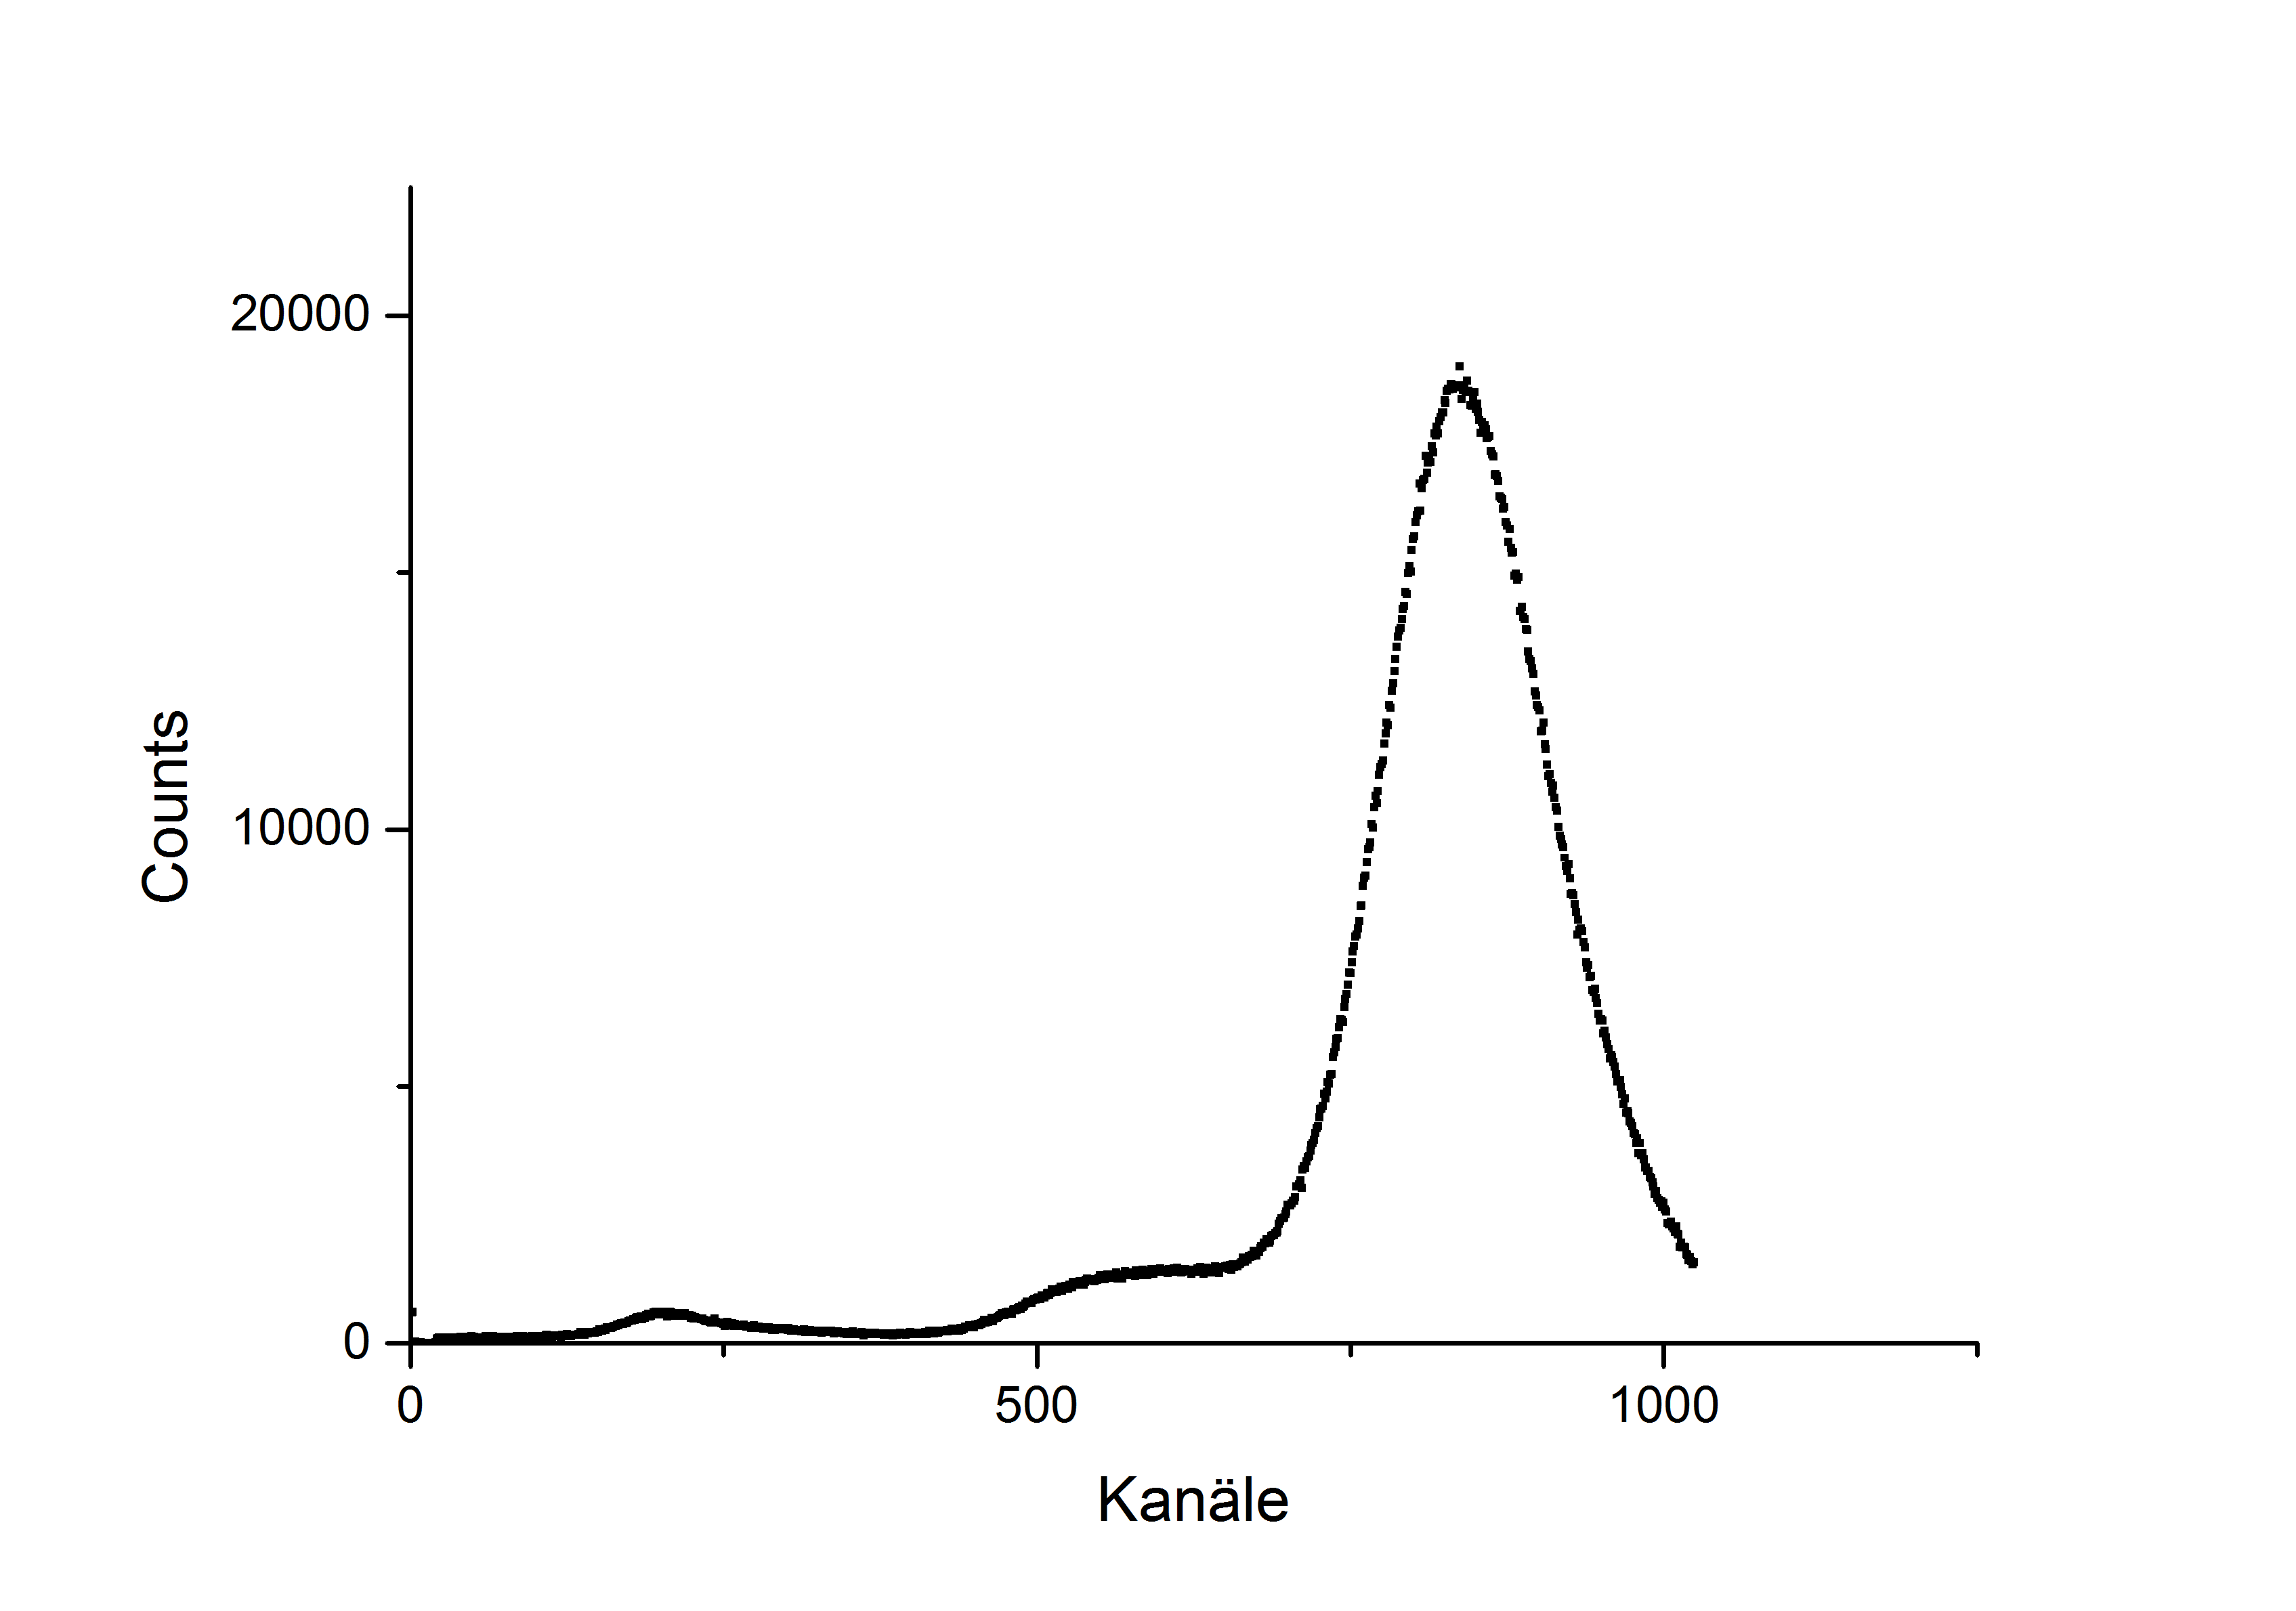
\includegraphics[scale=0.5]{coreszli}
\caption{Szintillator links, Öffnung $^{57}Co$ rechts}
\end{figure}
~\clearpage
\begin{figure}[h] 
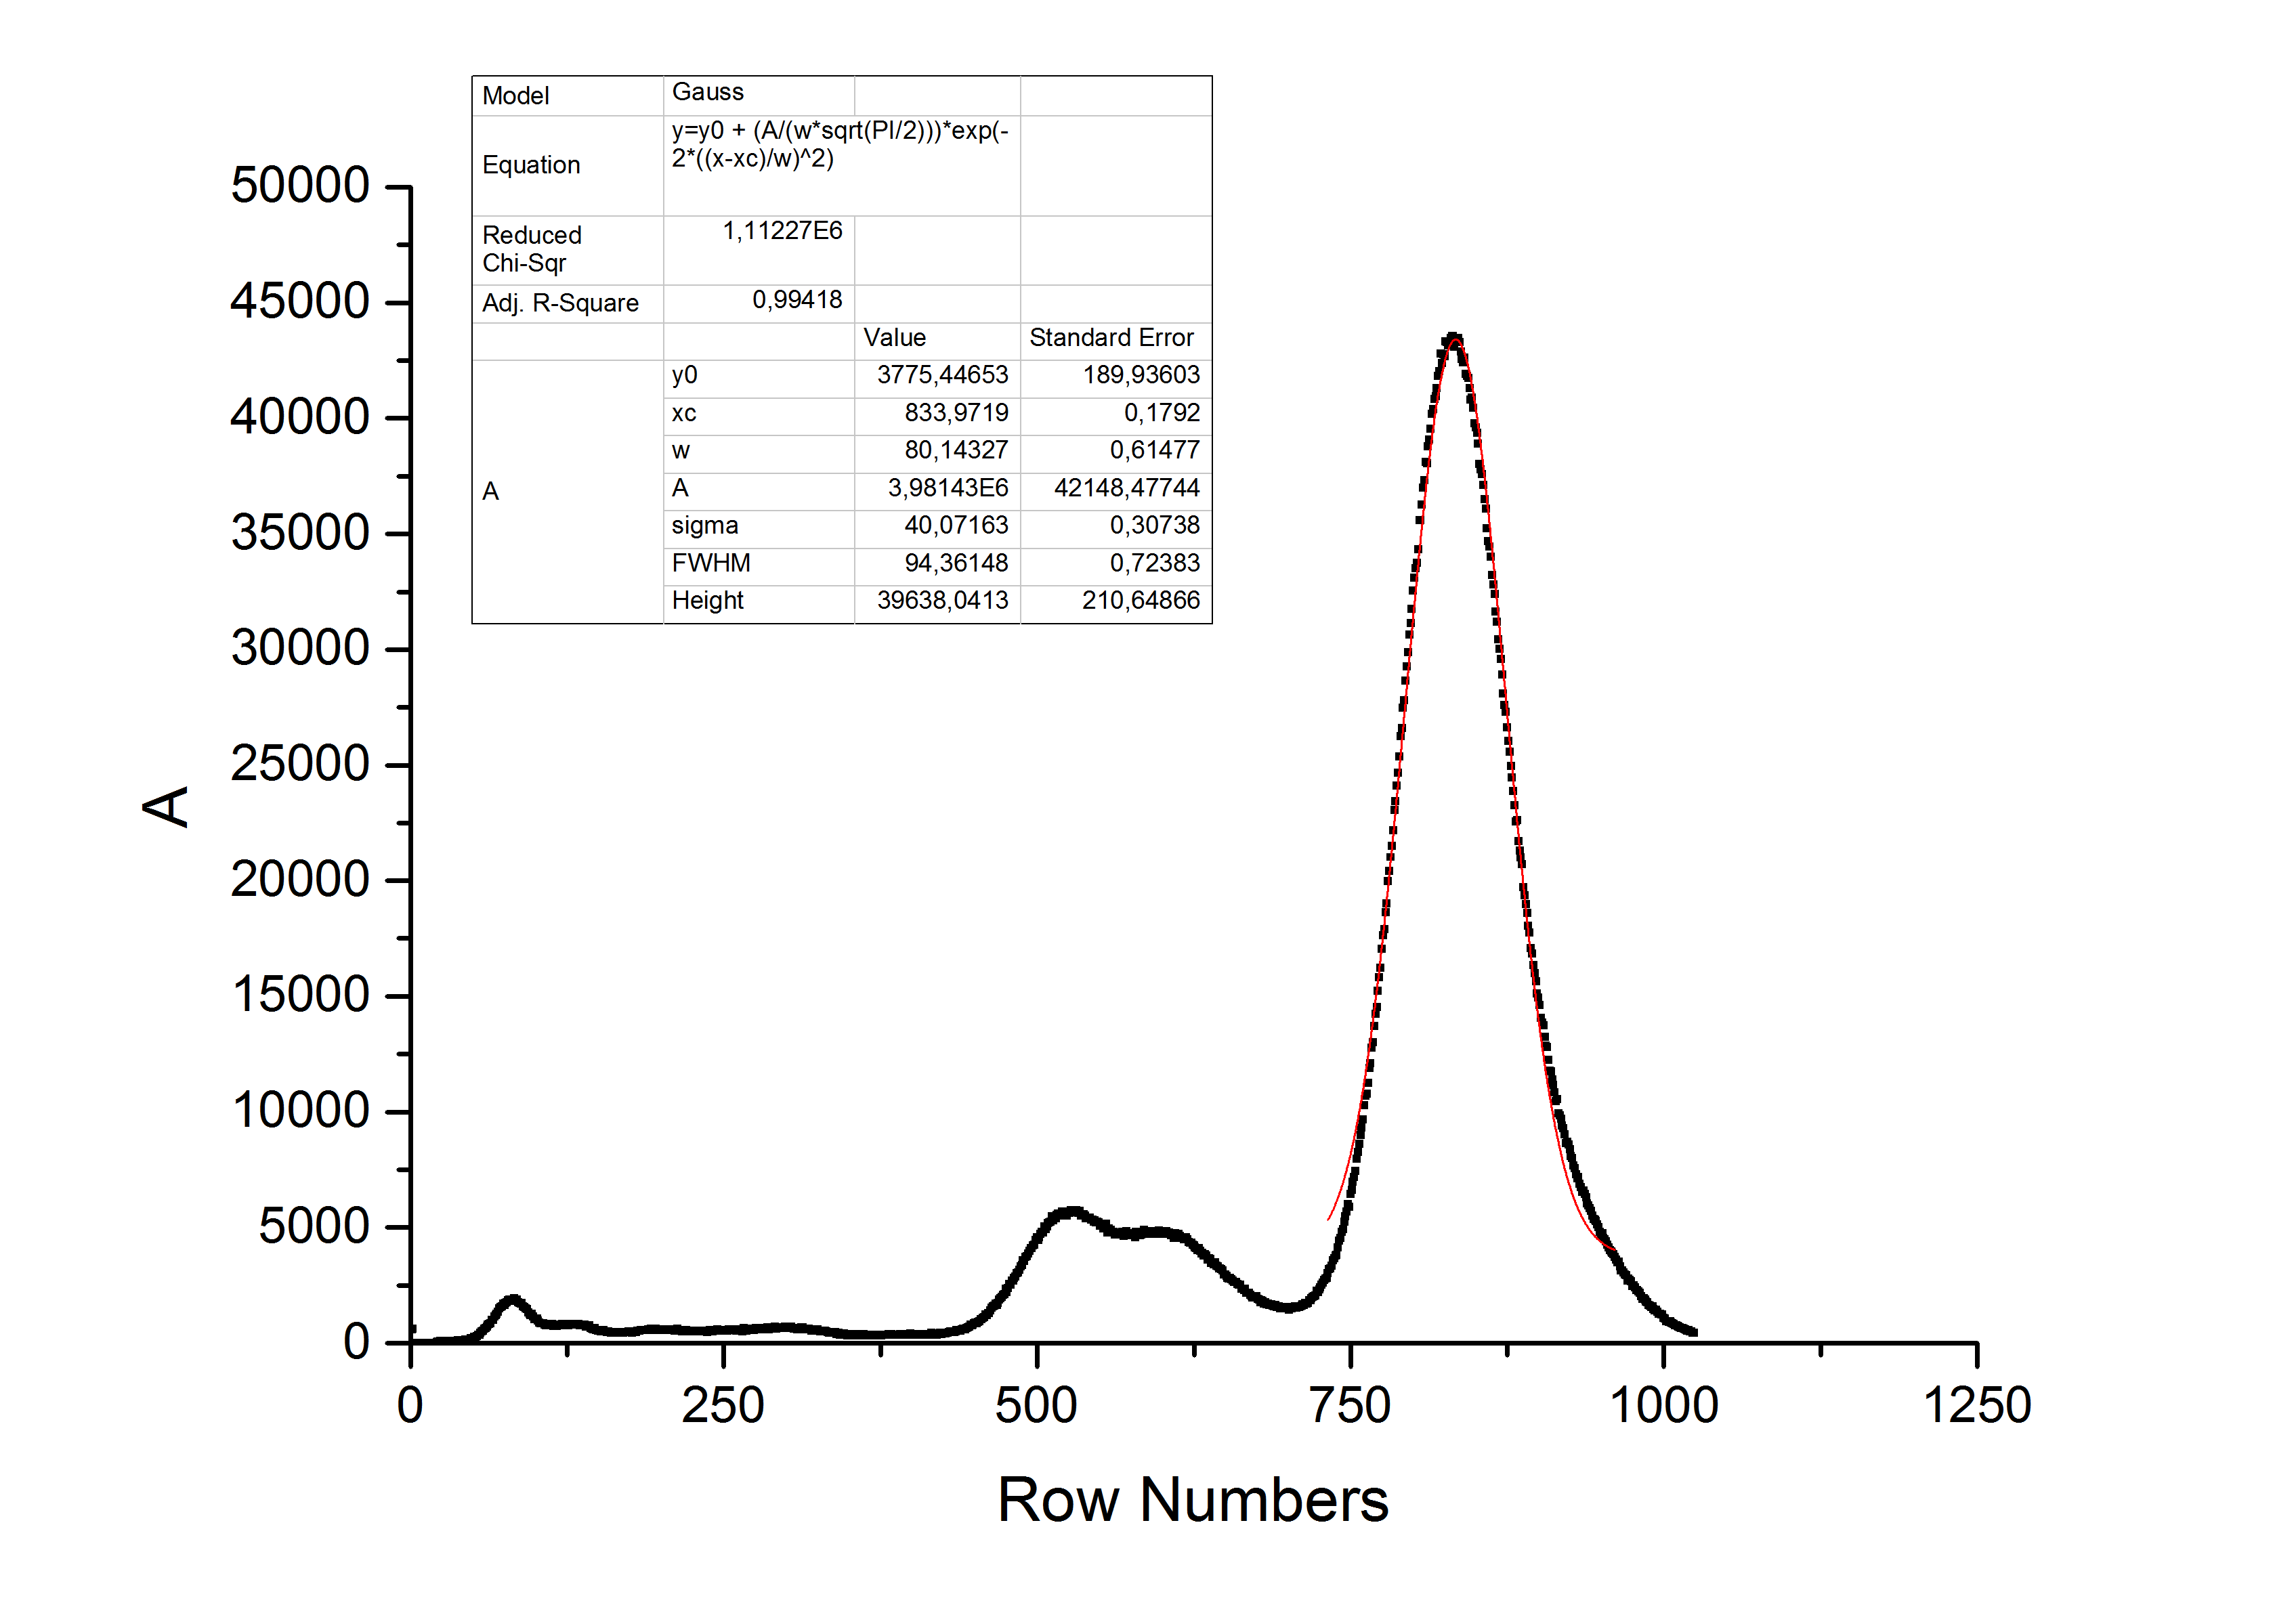
\includegraphics[scale=0.4]{coreszre}
\caption{Szintillator rechts, Öffnung $^{57}Co$ rechts}
\end{figure} 
Wir befanden die Ausrichtung \glqq Szintillator rechts, Öffnung rechts\grqq für die beste, da hier auch die Nebenpeaks gut ausgeprägt sichtbar waren. Aus diesem Grund führten wir für diese Messreihe eine Anpassung an dem bekannten 122,1 keV-Peak durch: Wir benutzten dabei einen Gauss-Fit. Das Ergebnis ist, wie am $\chi^2/dof$-Wert (dof steht für \glqq degrees of freedom\grqq, also Freiheitsgrade) ablesbar, sehr gut (der Wert ist sehr nah an 1). \\
Für $^{241}Am$ führten wir nur noch eine Messung mit der oben genannten Ausrichtung durch. Dabei erhielten wir folgendes Spektrum:
\begin{figure}[h] 
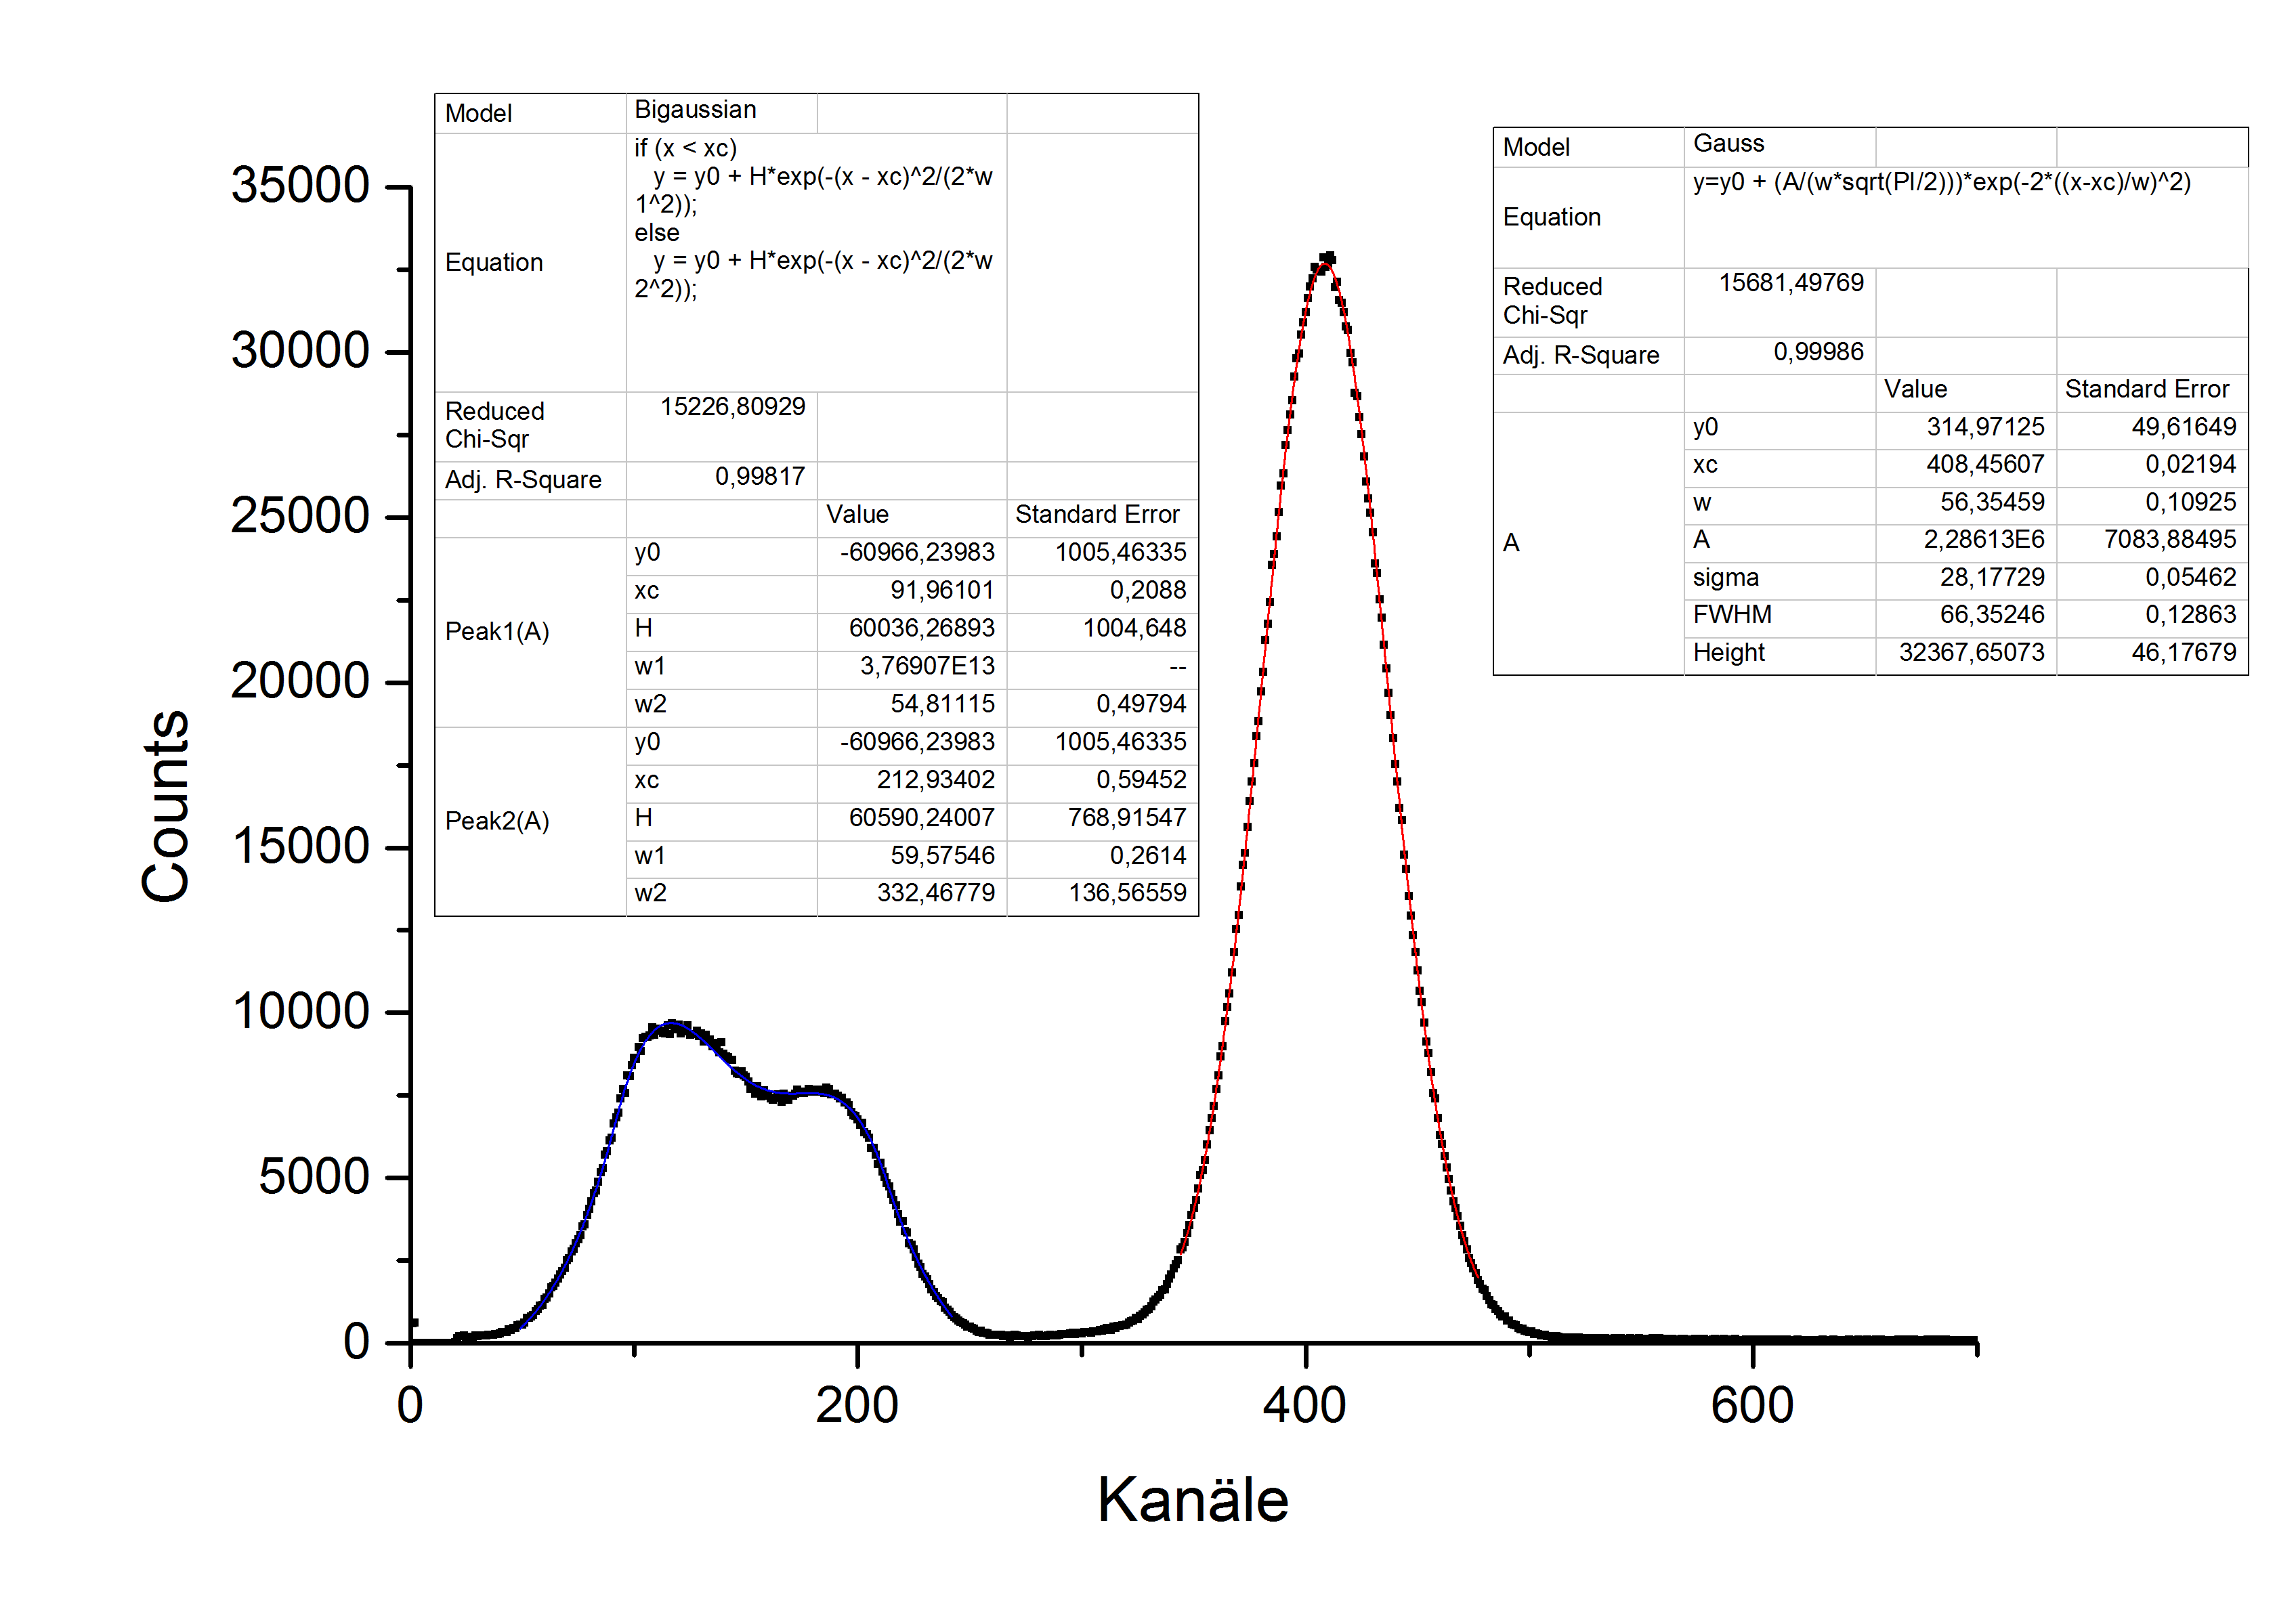
\includegraphics[scale=0.4]{amreszre}
\caption{Energiespektrum $^{241}Am$}
\end{figure}
\clearpage
Der 59,5 keV-Peak ist sehr klar auszumachen (roter Gauss-Fit). Bei niedrigeren Kanal-Zahlen lässt sich außerdem etwas wie ein doppelter Peak erahnen: Hierbei überschneiden sich die Signale des 26,3- und des 33,2 keV-Peaks. Aus diesem Grund wählten wir als Fitfunktion in diesem Bereich einen sogenannten \glqq Bigaussian\grqq, also eine doppelte Gauss-Funktion. Wie man an dem $\chi^2/dof$-Wert, welcher sehr nahe an 1 liegt, sieht, handelt es sich hierbei um eine gute Fitmethode. Selbiges gilt für den 59,5 keV-Peak.\\
Für die Zuordnung der Kanäle zu den bekannten Energien erhielten wir somit: \\
\begin{table}[htbp]
\caption{}
\begin{tabular}{rrr}

\multicolumn{1}{l}{Energie in keV} & \multicolumn{1}{l}{Kanal} & \multicolumn{1}{l}{Fehler Kanal} \\ 
26,3 & 92,0 & 0,2 \\ 
33,2 & 212,9 & 0,6 \\ 
59,5 & 408,46 & 0,02 \\ 
122,1 & 833,97 & 0,18 \\ 
\end{tabular}
\end{table} \\
Obwohl Kanäle diskret und äquidistant verteilt sind und ihnen natürliche Zahlen zugeordnet sind, haben wir uns entschlossen, hier den genauen Erwartungswert der Gauss-Fits mitsamt Fehler zu verwenden, um die Genauigkeit der Kalibrierung so groß wie möglich zu halten. Es ist anzumerken, dass aufgrund der Tatsache, dass hier eventuelle Fehler der involvierten Teile des Aufbaus vernachlässigt wurden, der Fehler größer sein dürfte als aus dem Fit berechnet. \\
Die Zuordnung Kanal - Energie erfolgt im MCA linear. Aus diesem Grund benutzten wir einen linearen Fit, welcher folgendermaßen aussieht: \\
\begin{figure}[h]
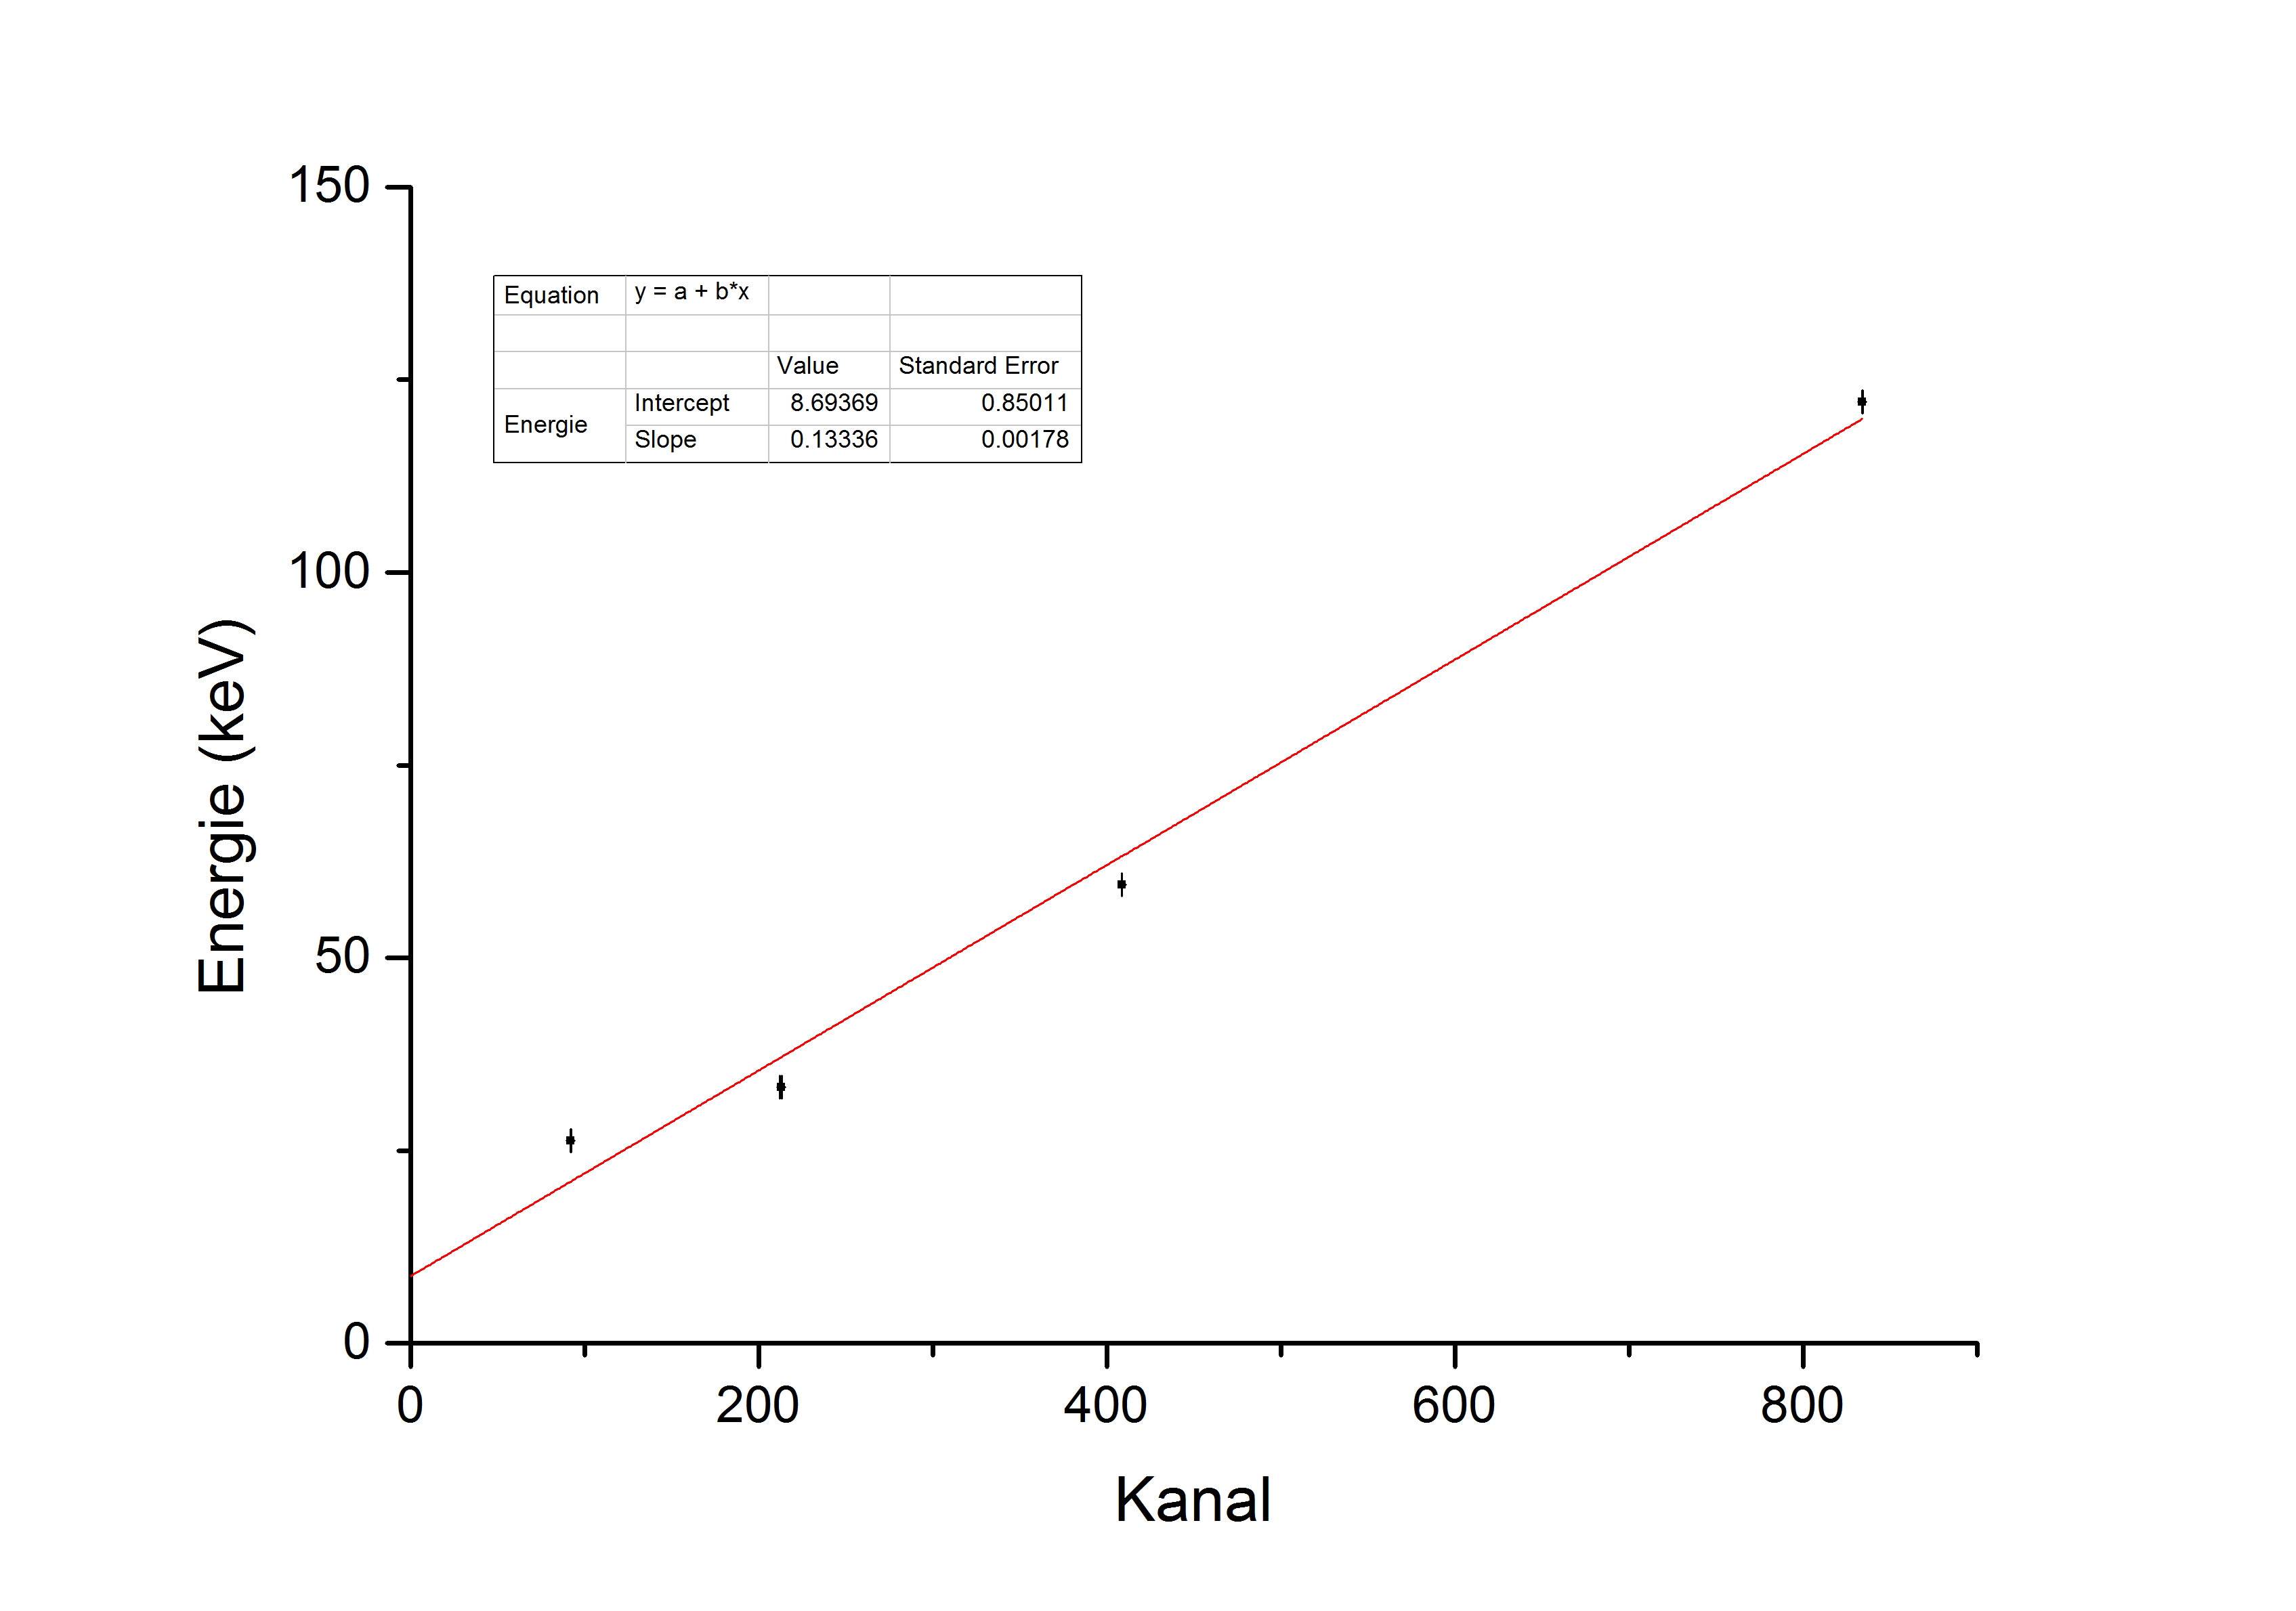
\includegraphics[scale=0.5]{energiefit}
\caption{Energiekalibrierung}
\end{figure}\\
Die Werte liegen nicht genau auf einer Geraden, was angesichts der Tatsache, dass die Fehler vernachlässigt wurden und jedes Spektrum nur einmal vermessen wurde, nicht überraschend ist. 
\subsection{Verzögerte Koinzidenzen}
\subsubsection{Zeitkalibrierung des TAC}
Für die Messung der verzögerten Koinzidenzen haben wir wie auch für die nachfolgende Messung der zufälligen Koinzidenzen einen \glqq Time-to-Amplitude Converter\grqq (TAC) verwendet. Dieser transformiert eine Zeitverzögerung in eine Spannung, welche vom MCA gemessen und einem Kanal zugeordnet werden kann. Um einen Zusammenhang zwischen der Zeitverzögerung und dem der Spannung zugeordneten Kanal bestimmen zu können, stellten wir unterschiedliche Verzögerungen ein und schrieben uns den zugeordneten Kanal auf (für die Messwerte s. Anhang). Dabei entschieden wir uns, obwohl für manche Verzögerungen nicht nur bei einem Kanal ein Signal registriert wurde, sondern bei zweien, jeweils das Signal mit der größeren Anzahl an Counts zu verwenden (unterstrichene Werte im Anhang). Schließlich trugen wir die Verzögerungen über die Kanäle auf und verwendeten, um eine Kalibrierung zu bekommen, einen linearen Fit:\\
\begin{figure}[h]
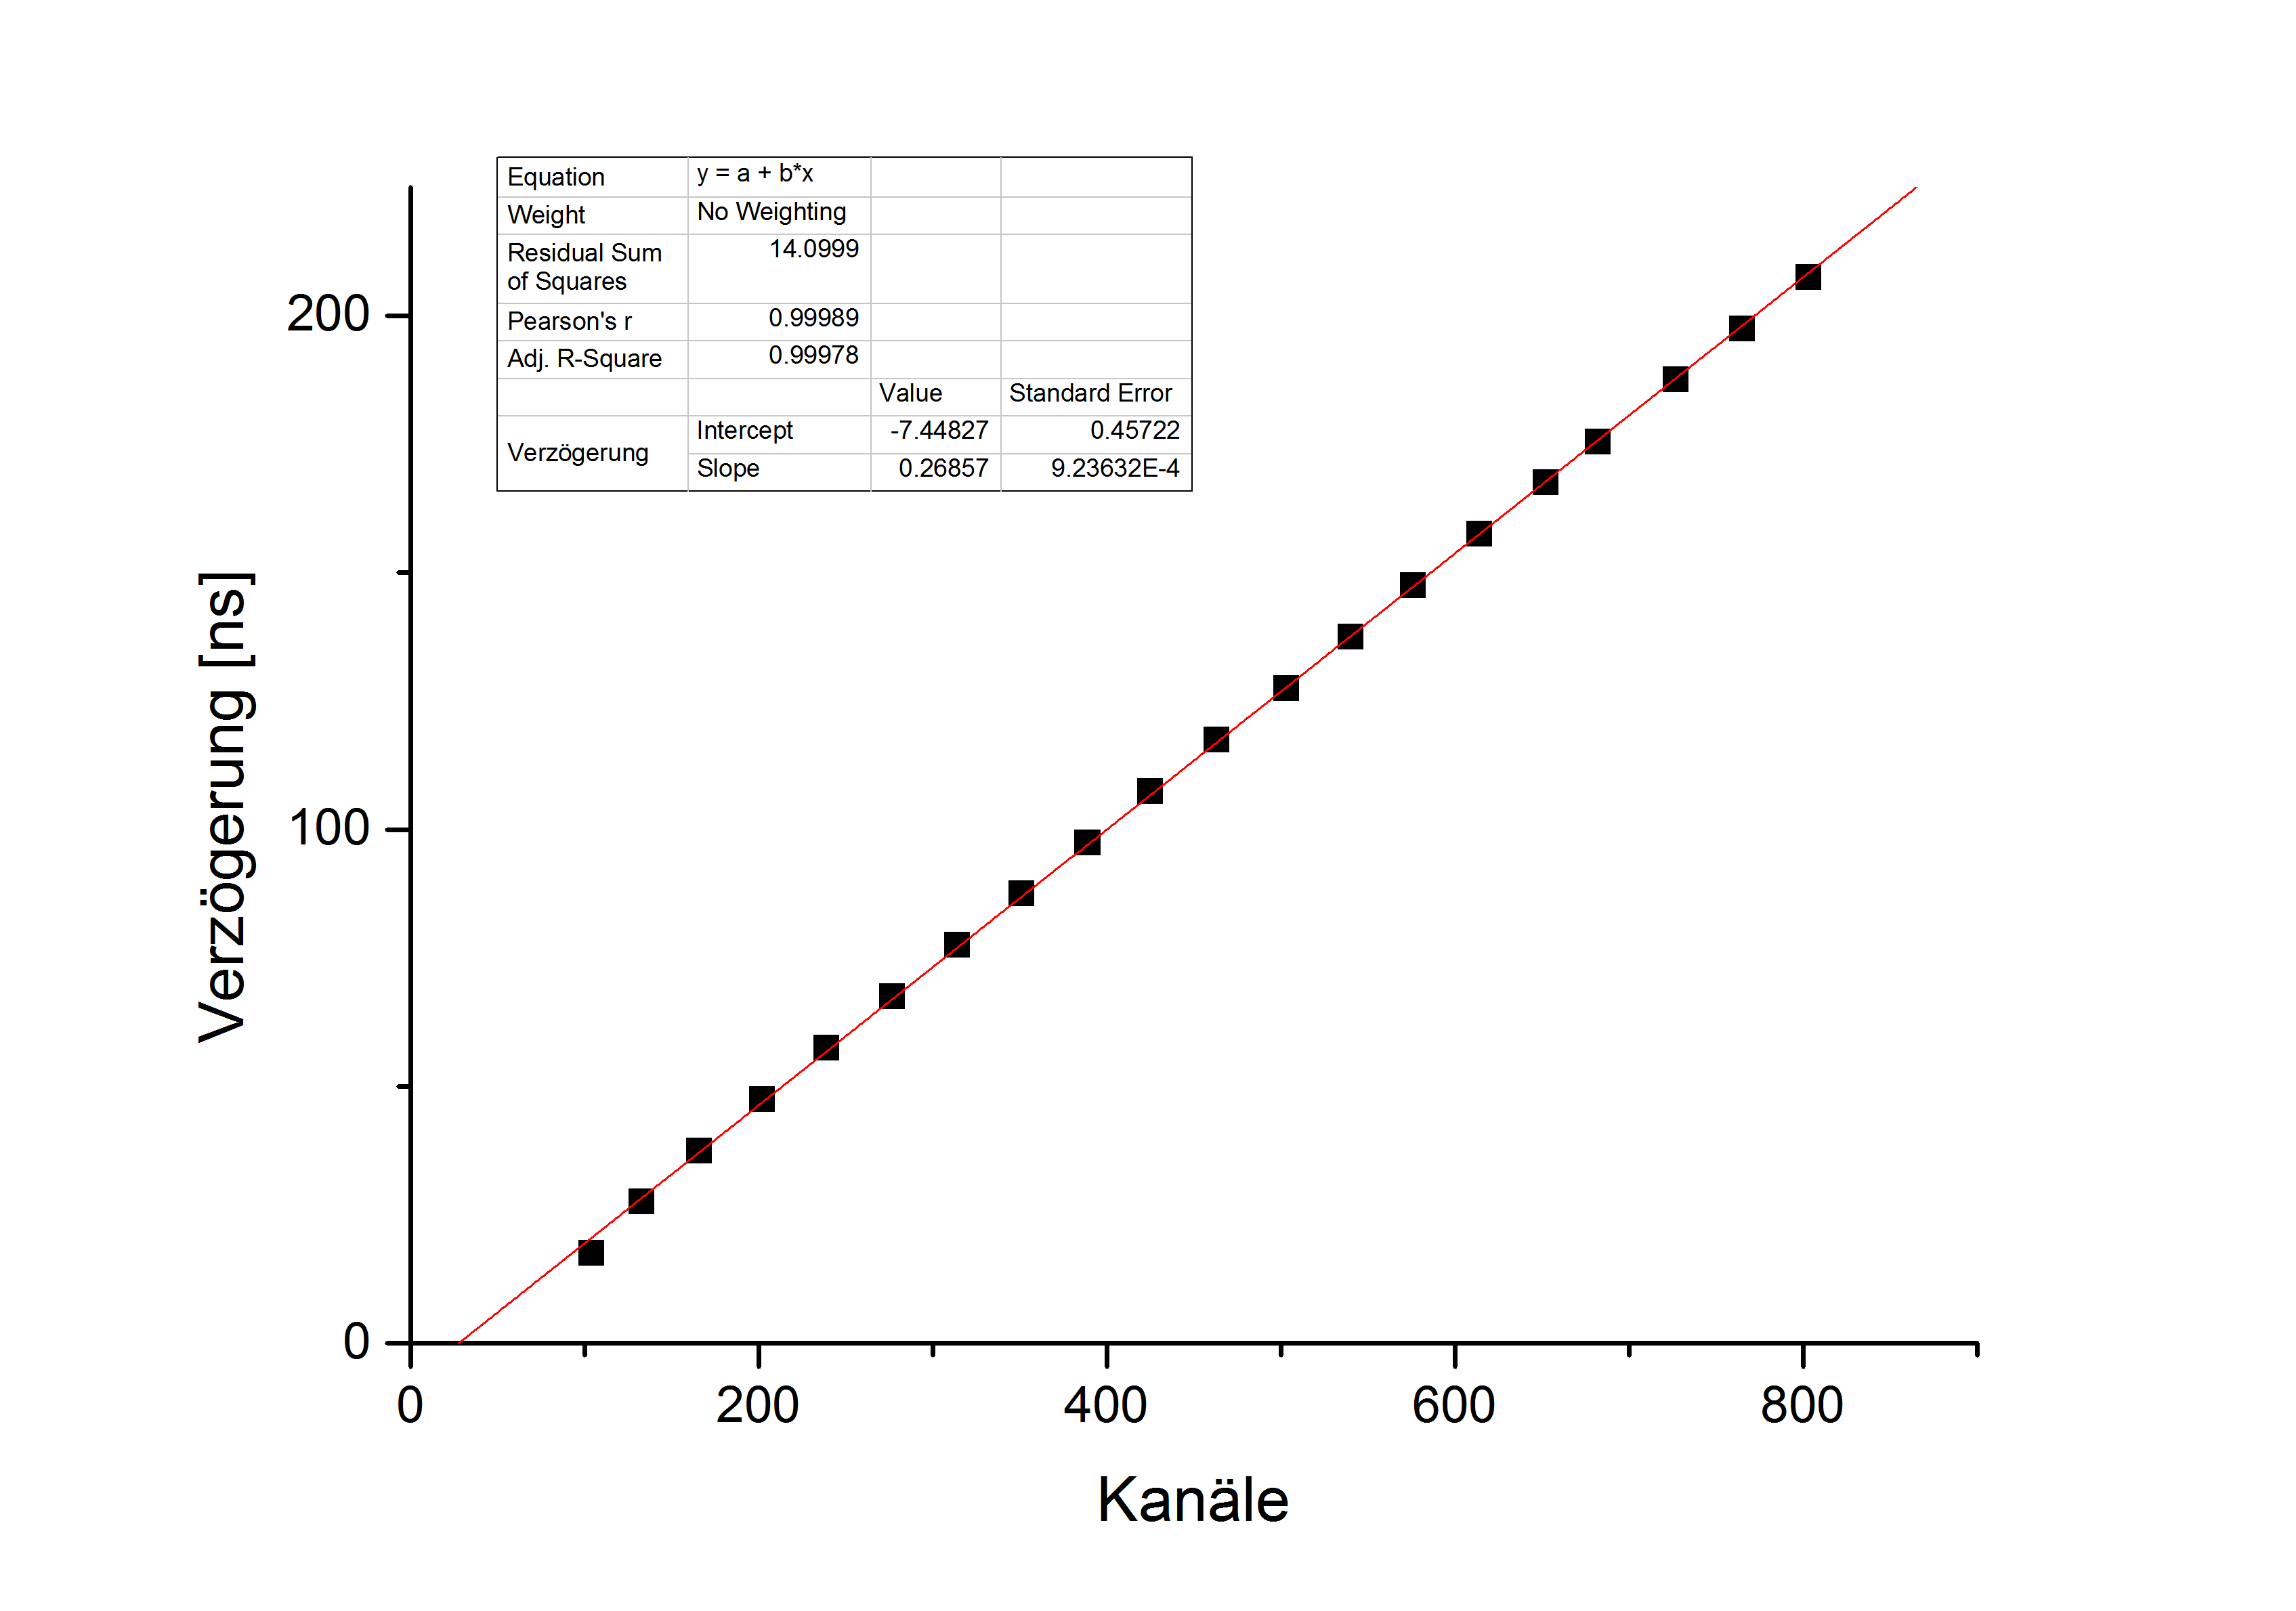
\includegraphics[scale=0.5]{delayfit}
\caption{Kalibrierung der Verzögerung}
\end{figure}\\
Dabei erhielten wir für die Steigung:\\
$b=(0,2686\pm0,0009)\frac{ns}{Kanal}$\\
Wie der negative Offset vermuten lässt, ist allerdings die tatsächliche Verzögerung größer als die durch das Gerät und die verwendeten Kabel verwendete. Dies ist für unsere Auswertung aber nicht von Bedeutung, da nur die Steigung eine Rolle spielt. Für diese ist der Fehler wohl zu klein berechnet, da für die eingestellten Verzögerungen keine Fehler angenommen wurden. Der Fit selbst ist mit einem $\chi^{2}/dof$ von nahezu 1 sehr gut. \\
\subsubsection{Halbwertszeitbestimmung - Exponentielle Methode}
Aufgrund möglicher zufälliger Koinzidenzen, welche in diesem Versuch den Untergrund ausmachen, musste unsere Messung der verzögerten Koinzidenzen von diesen bereinigt werden. Um das tun zu können, haben wir aufgrund der unterschiedlichen Messdauer die Counts der Messung der zufälligen Koinzidenzen jeweils mit einem Vorfaktor $\frac{t_{v}}{t_{z}}$ multipliziert (dabei ist die Messdauer der zufällgen Koinzidenzen $t_{z}=6333 s$ und die der verzögerten Koinzidenzen $t_{v}=58886 s$).\\
$\Rightarrow N=N_{v}-\frac{t_{v}}{t_{z}}*N_{z}$\\
Der so erstellte Graph sollte für den ansteigenden Teil mit einer Exponentialfunktion der Form $N=y_{0}+A*e^{R_{0}*Kanal}$ modelliert werden. \\
\begin{figure}[h]
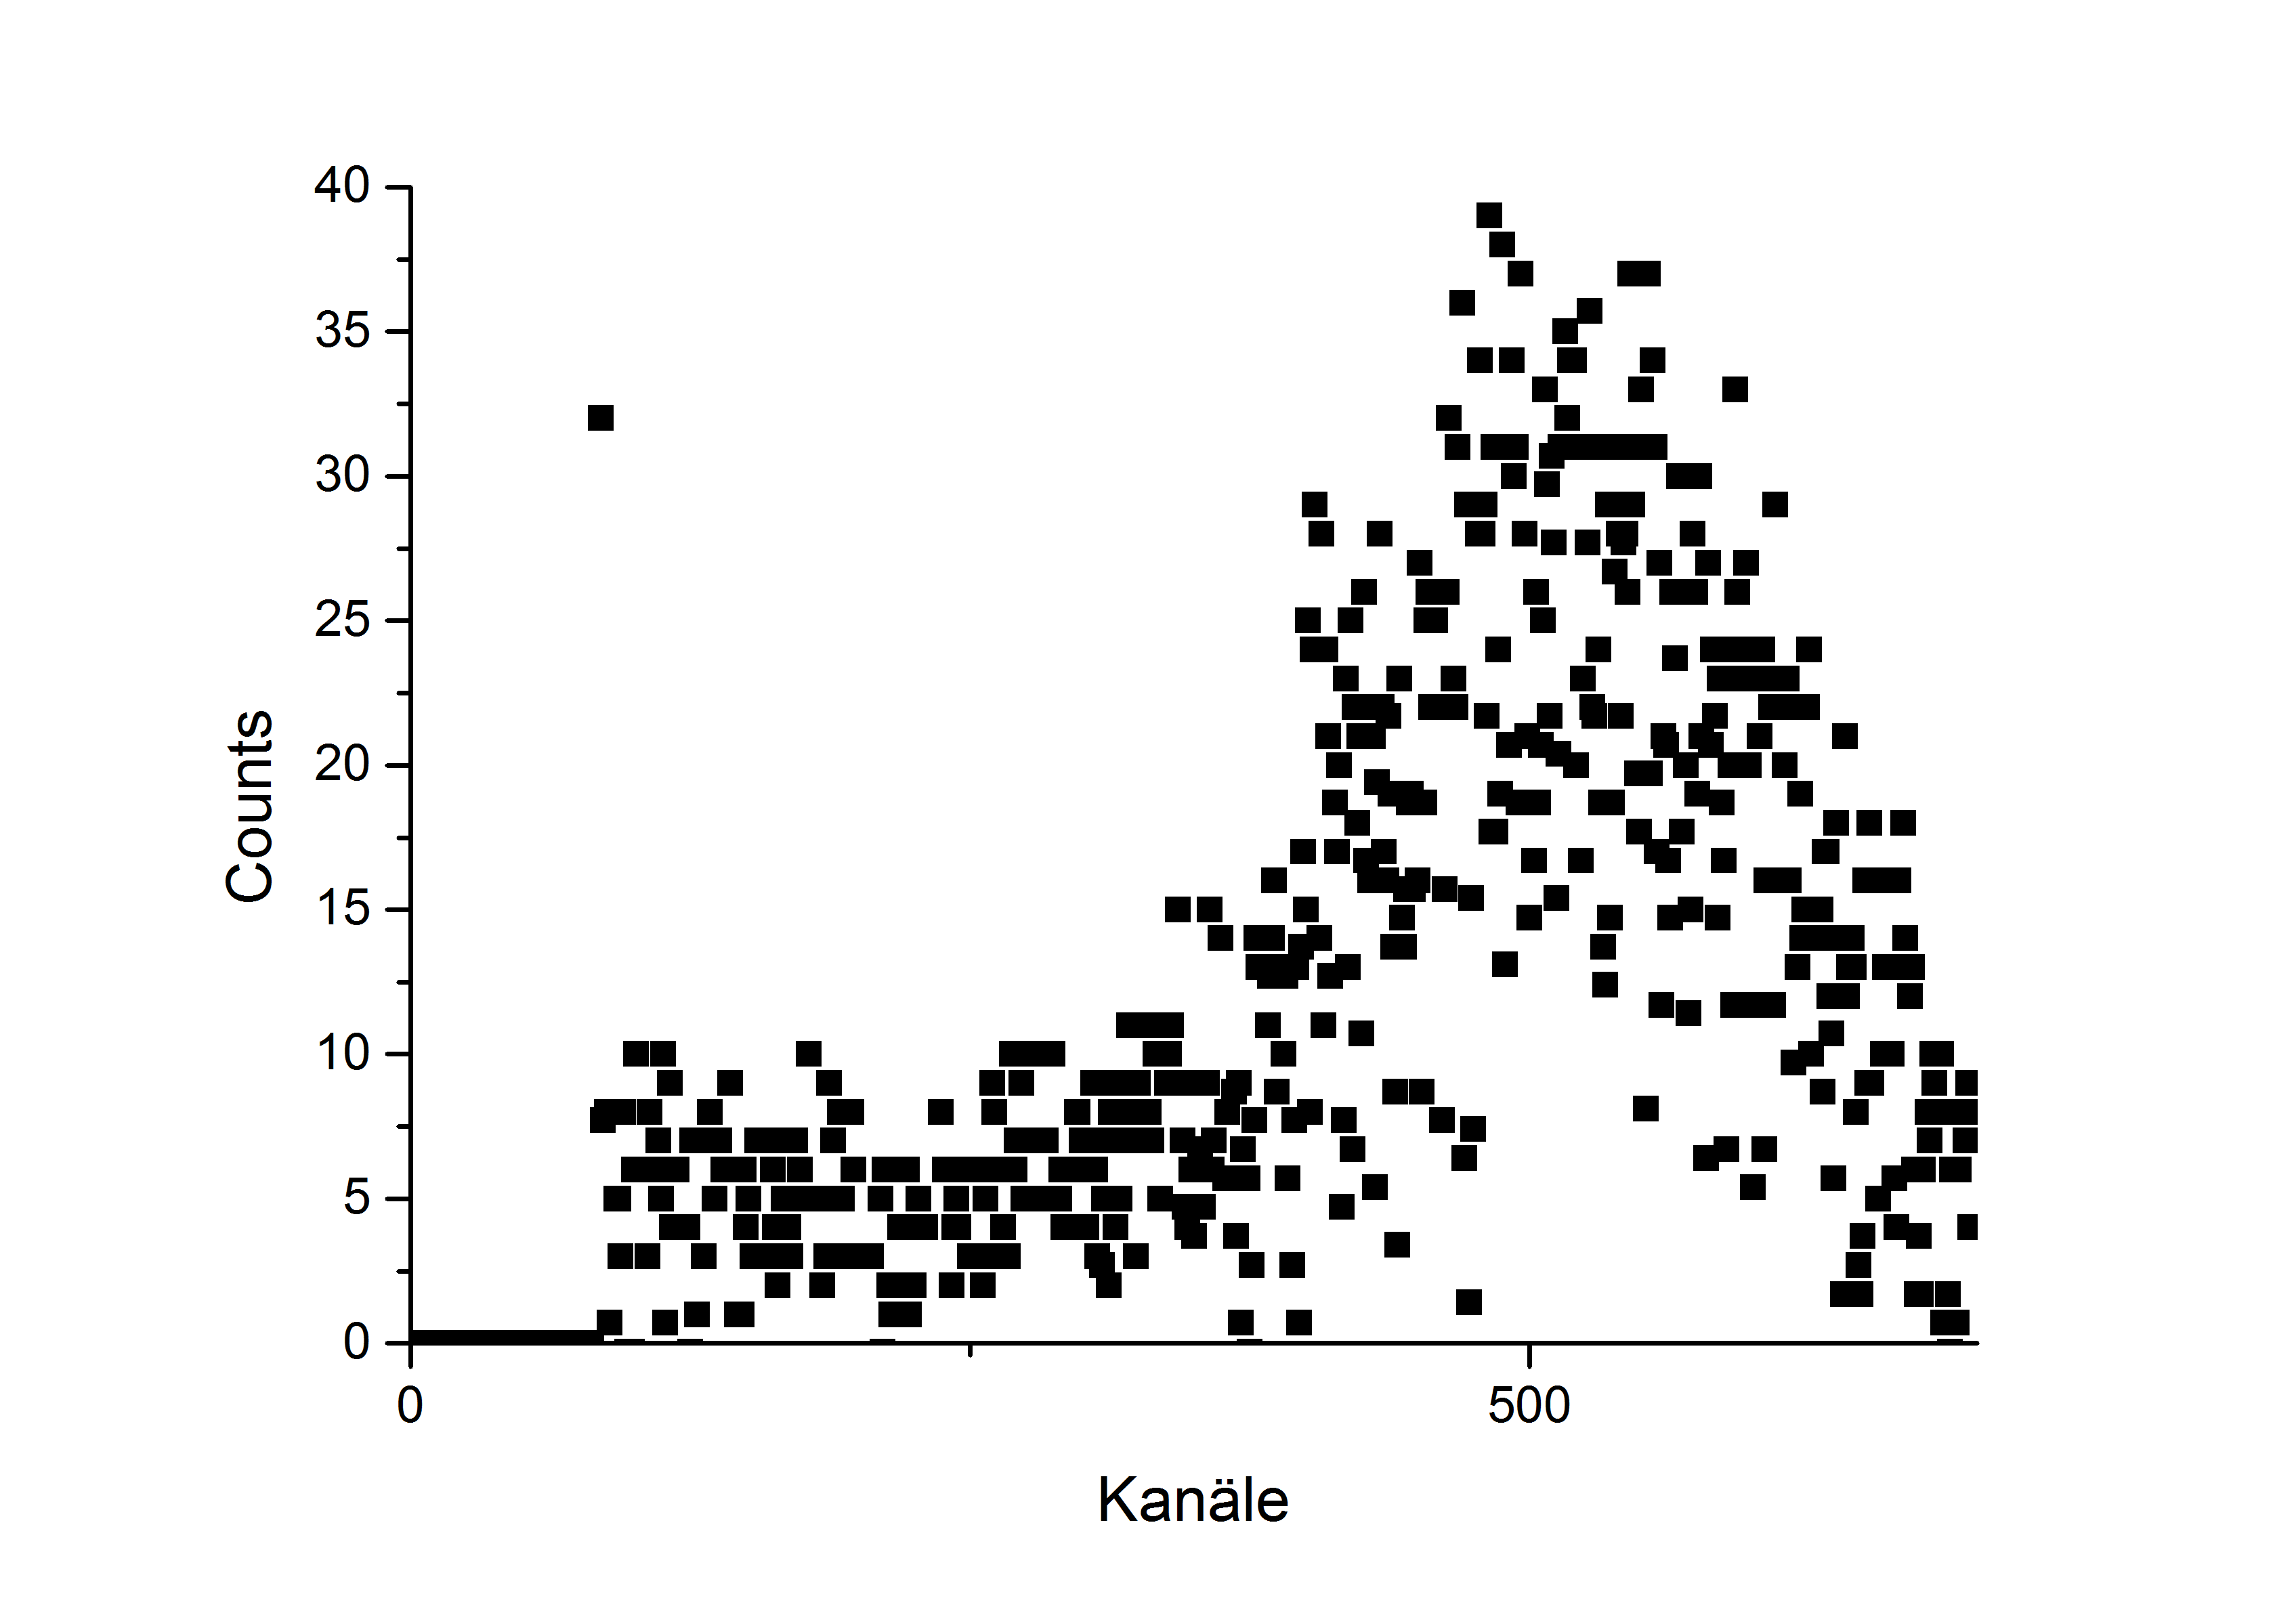
\includegraphics[scale=0.6]{urspruenglich}
\caption{Von zufälligen Koinzidenzen bereinigte Messung.}
\end{figure}\\
Wie man sieht, ist die Streuung zwischen nah beieinander liegenden Kanälen groß. Ein Grund hierfür könnte sein, dass die Messung der zufälligen Koinzidenzen nicht einmal zwei Stunden dauerte, was eine sehr niedrige Dauer für eine solche Messung ist. Um die enorme Streuung etwas zu reduzieren, entschlossen wir uns, jeweils 5 Kanäle zusammenzufassen nach der Methode:\\ $N_{i_{neu}}=\frac{N_{i-2}+N_{i-1}+N_{i}+N_{i+1}+N_{i+2}}{5}$\\
\glqq i\grqq steht hierbei für die Zahl eines Kanals. Für die obersten und die untersten zwei Kanäle behielten wir den ursprünglichen Wert. Da diese keine große Rolle spielen, sollte dies kein Problem darstellen.\\
Insgesamt ergab sich somit die Formel:\\
\[N_{i}=0,2*(N_{v_{i-2}}+...+N_{v_{i+2}}-\frac{t_{v}}{t_{z}}*(N_{z_{i-2}}+...+N_{z_{i+2}}))\]
\clearpage
\begin{figure}[h]
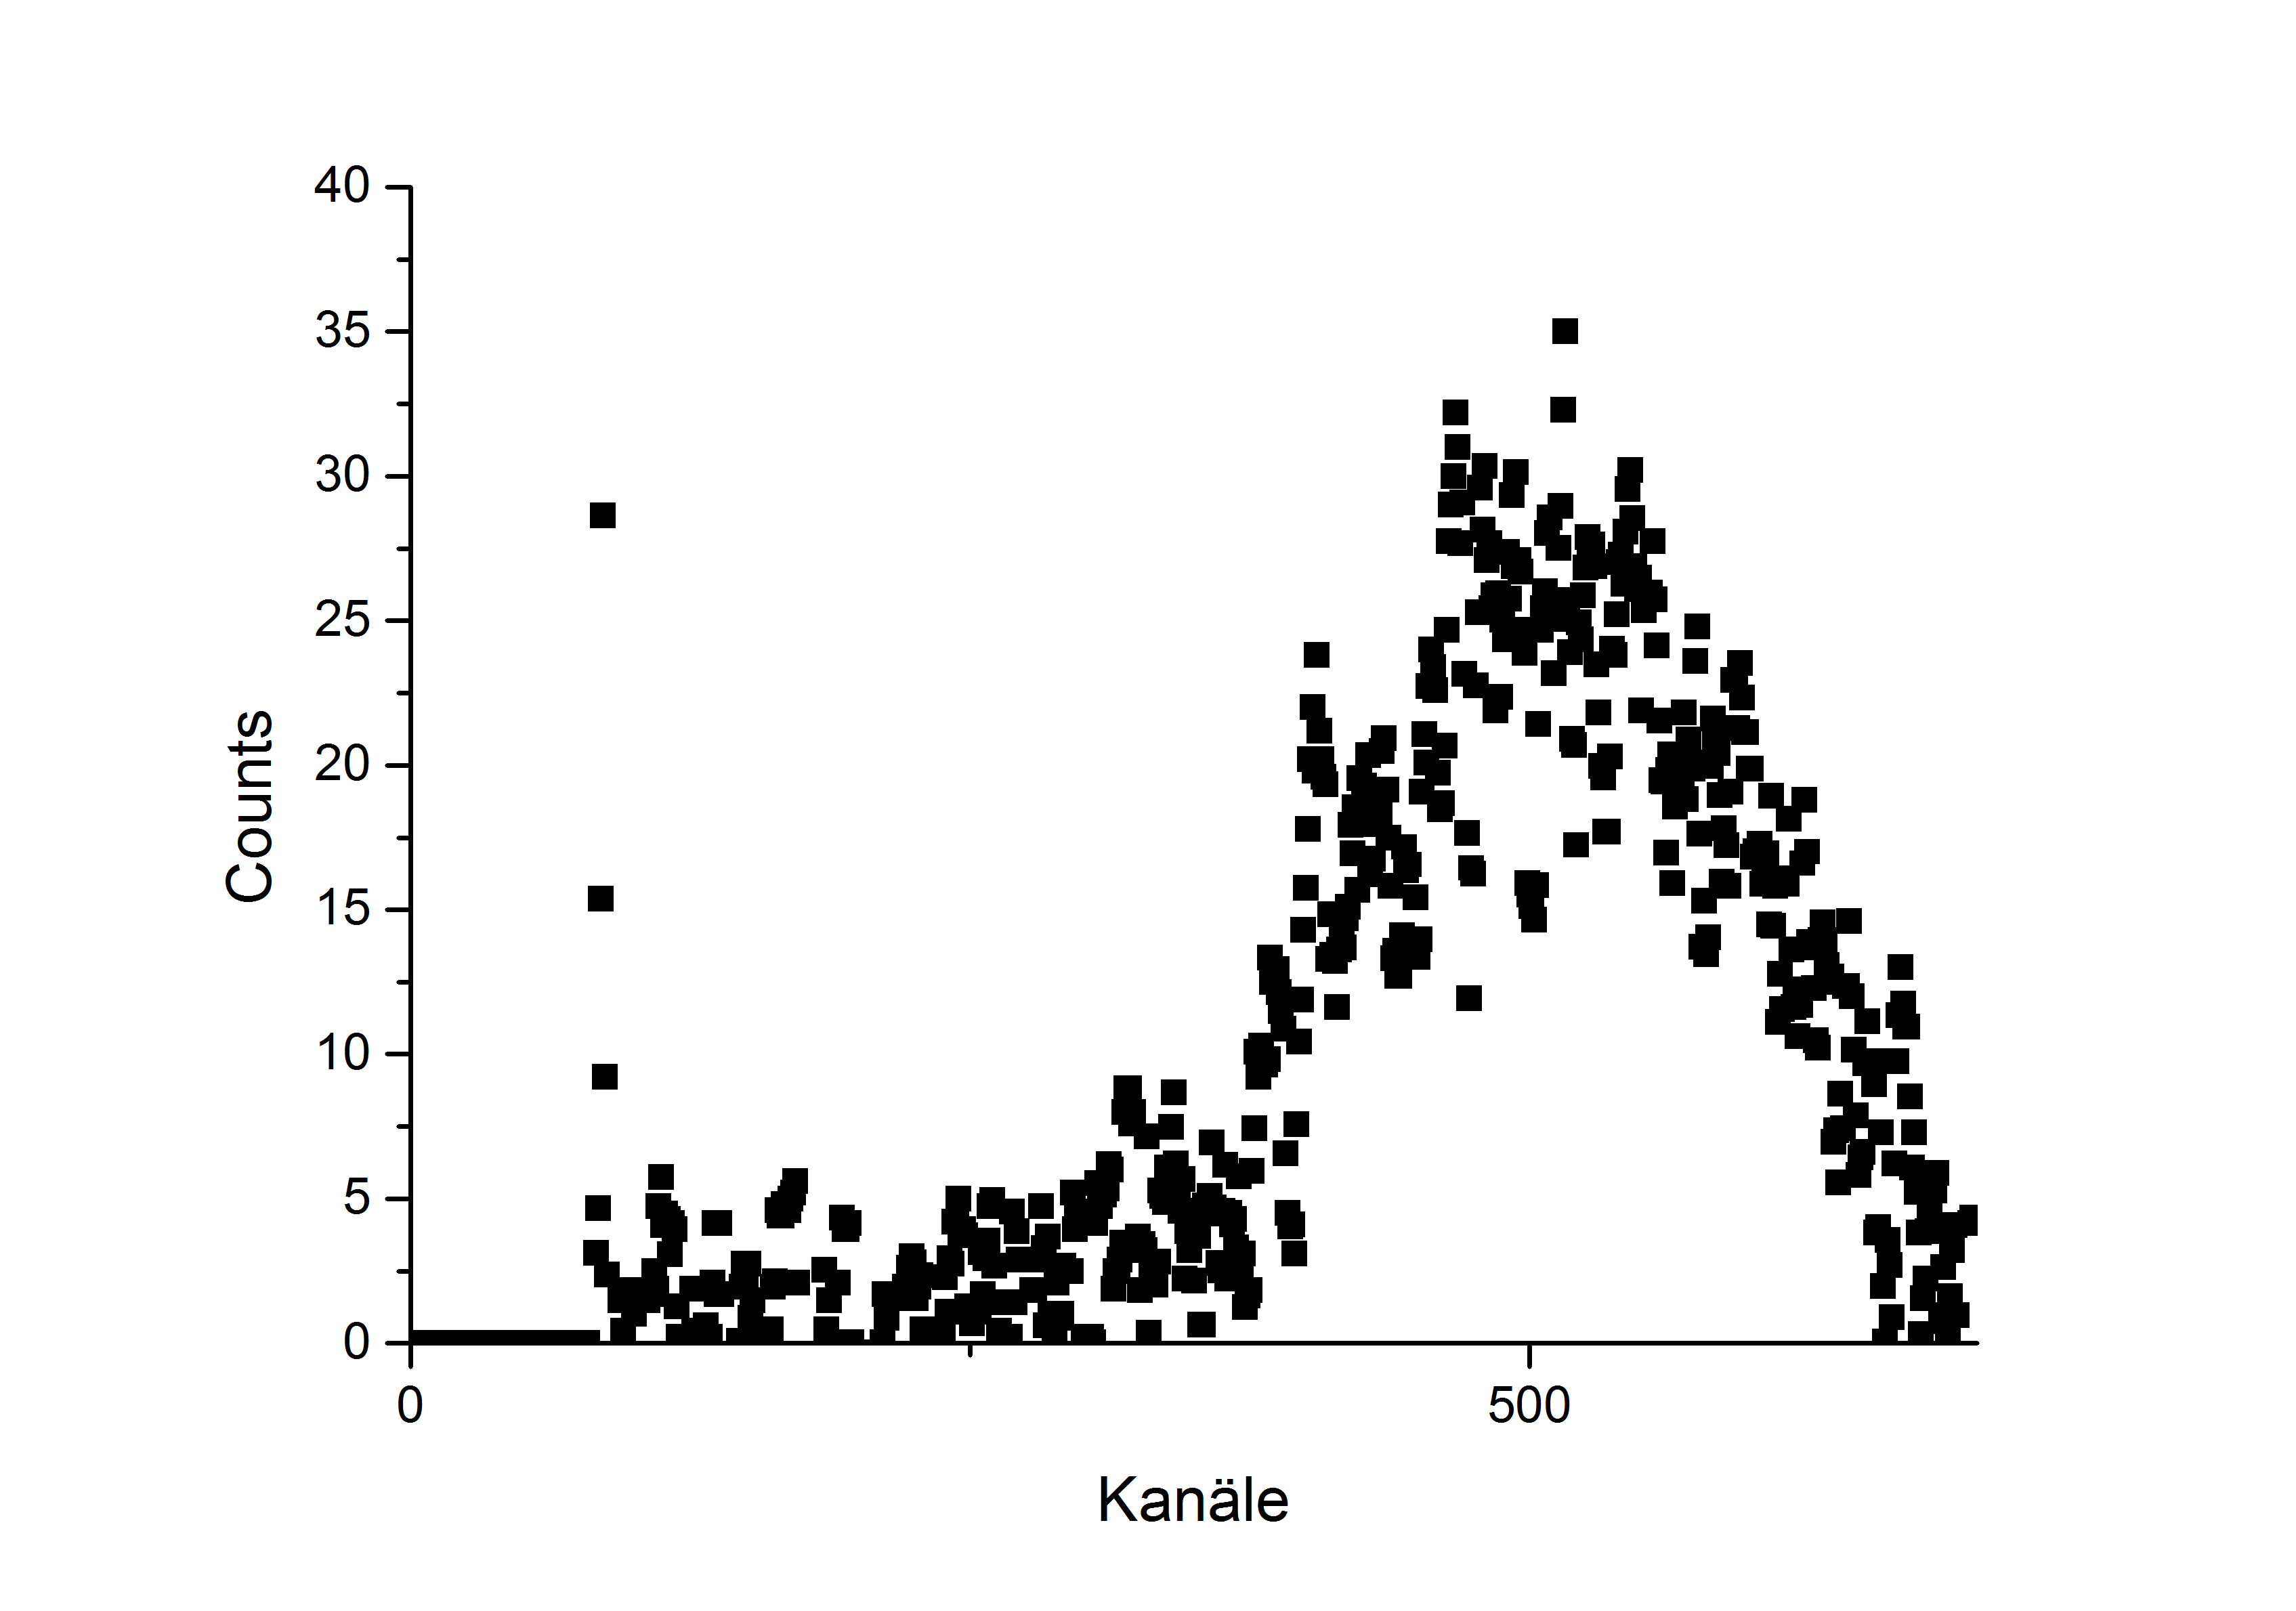
\includegraphics[scale=0.6]{korrigiert}
\caption{Nach neuer Methode bestimmtes Spektrum.}
\end{figure}
Es ist offensichtlich, dass durch die oben erklärte Methode eine Reduzierung der Streuung erreicht werden konnte.\\
Beide Messungen können durch eine Poissonverteilung modelliert werden. Mit Gauss'scher Fehlerfortpflanzung ergibt sich:\\
\[\Rightarrow s_{N_{i}}=0,2*\sqrt{(s_{N_{v_{i-2}}})^{2}+...(s_{N_{v_{i+2}}})^{2}+(\frac{t_{v}}{t_{z}})^{2}*((s_{N_{z_{i-2}}})^{2}+...+(s_{N_{z_{i+2}}})^{2}}\]
\[=0,2*\sqrt{N_{v_{i-2}}+...+N_{v_{i+2}}+(\frac{t_{v}}{t_{z}})^{2}*(N_{z_{i-2}}+...+N_{z_{i+2}})}\]\\
Für die ersten beiden und die letzten Kanäle analog berechnet, bloß ohne die Summen.\\
Somit sieht das Spektrum folgendermaßen aus:
\clearpage
\begin{figure}[h]
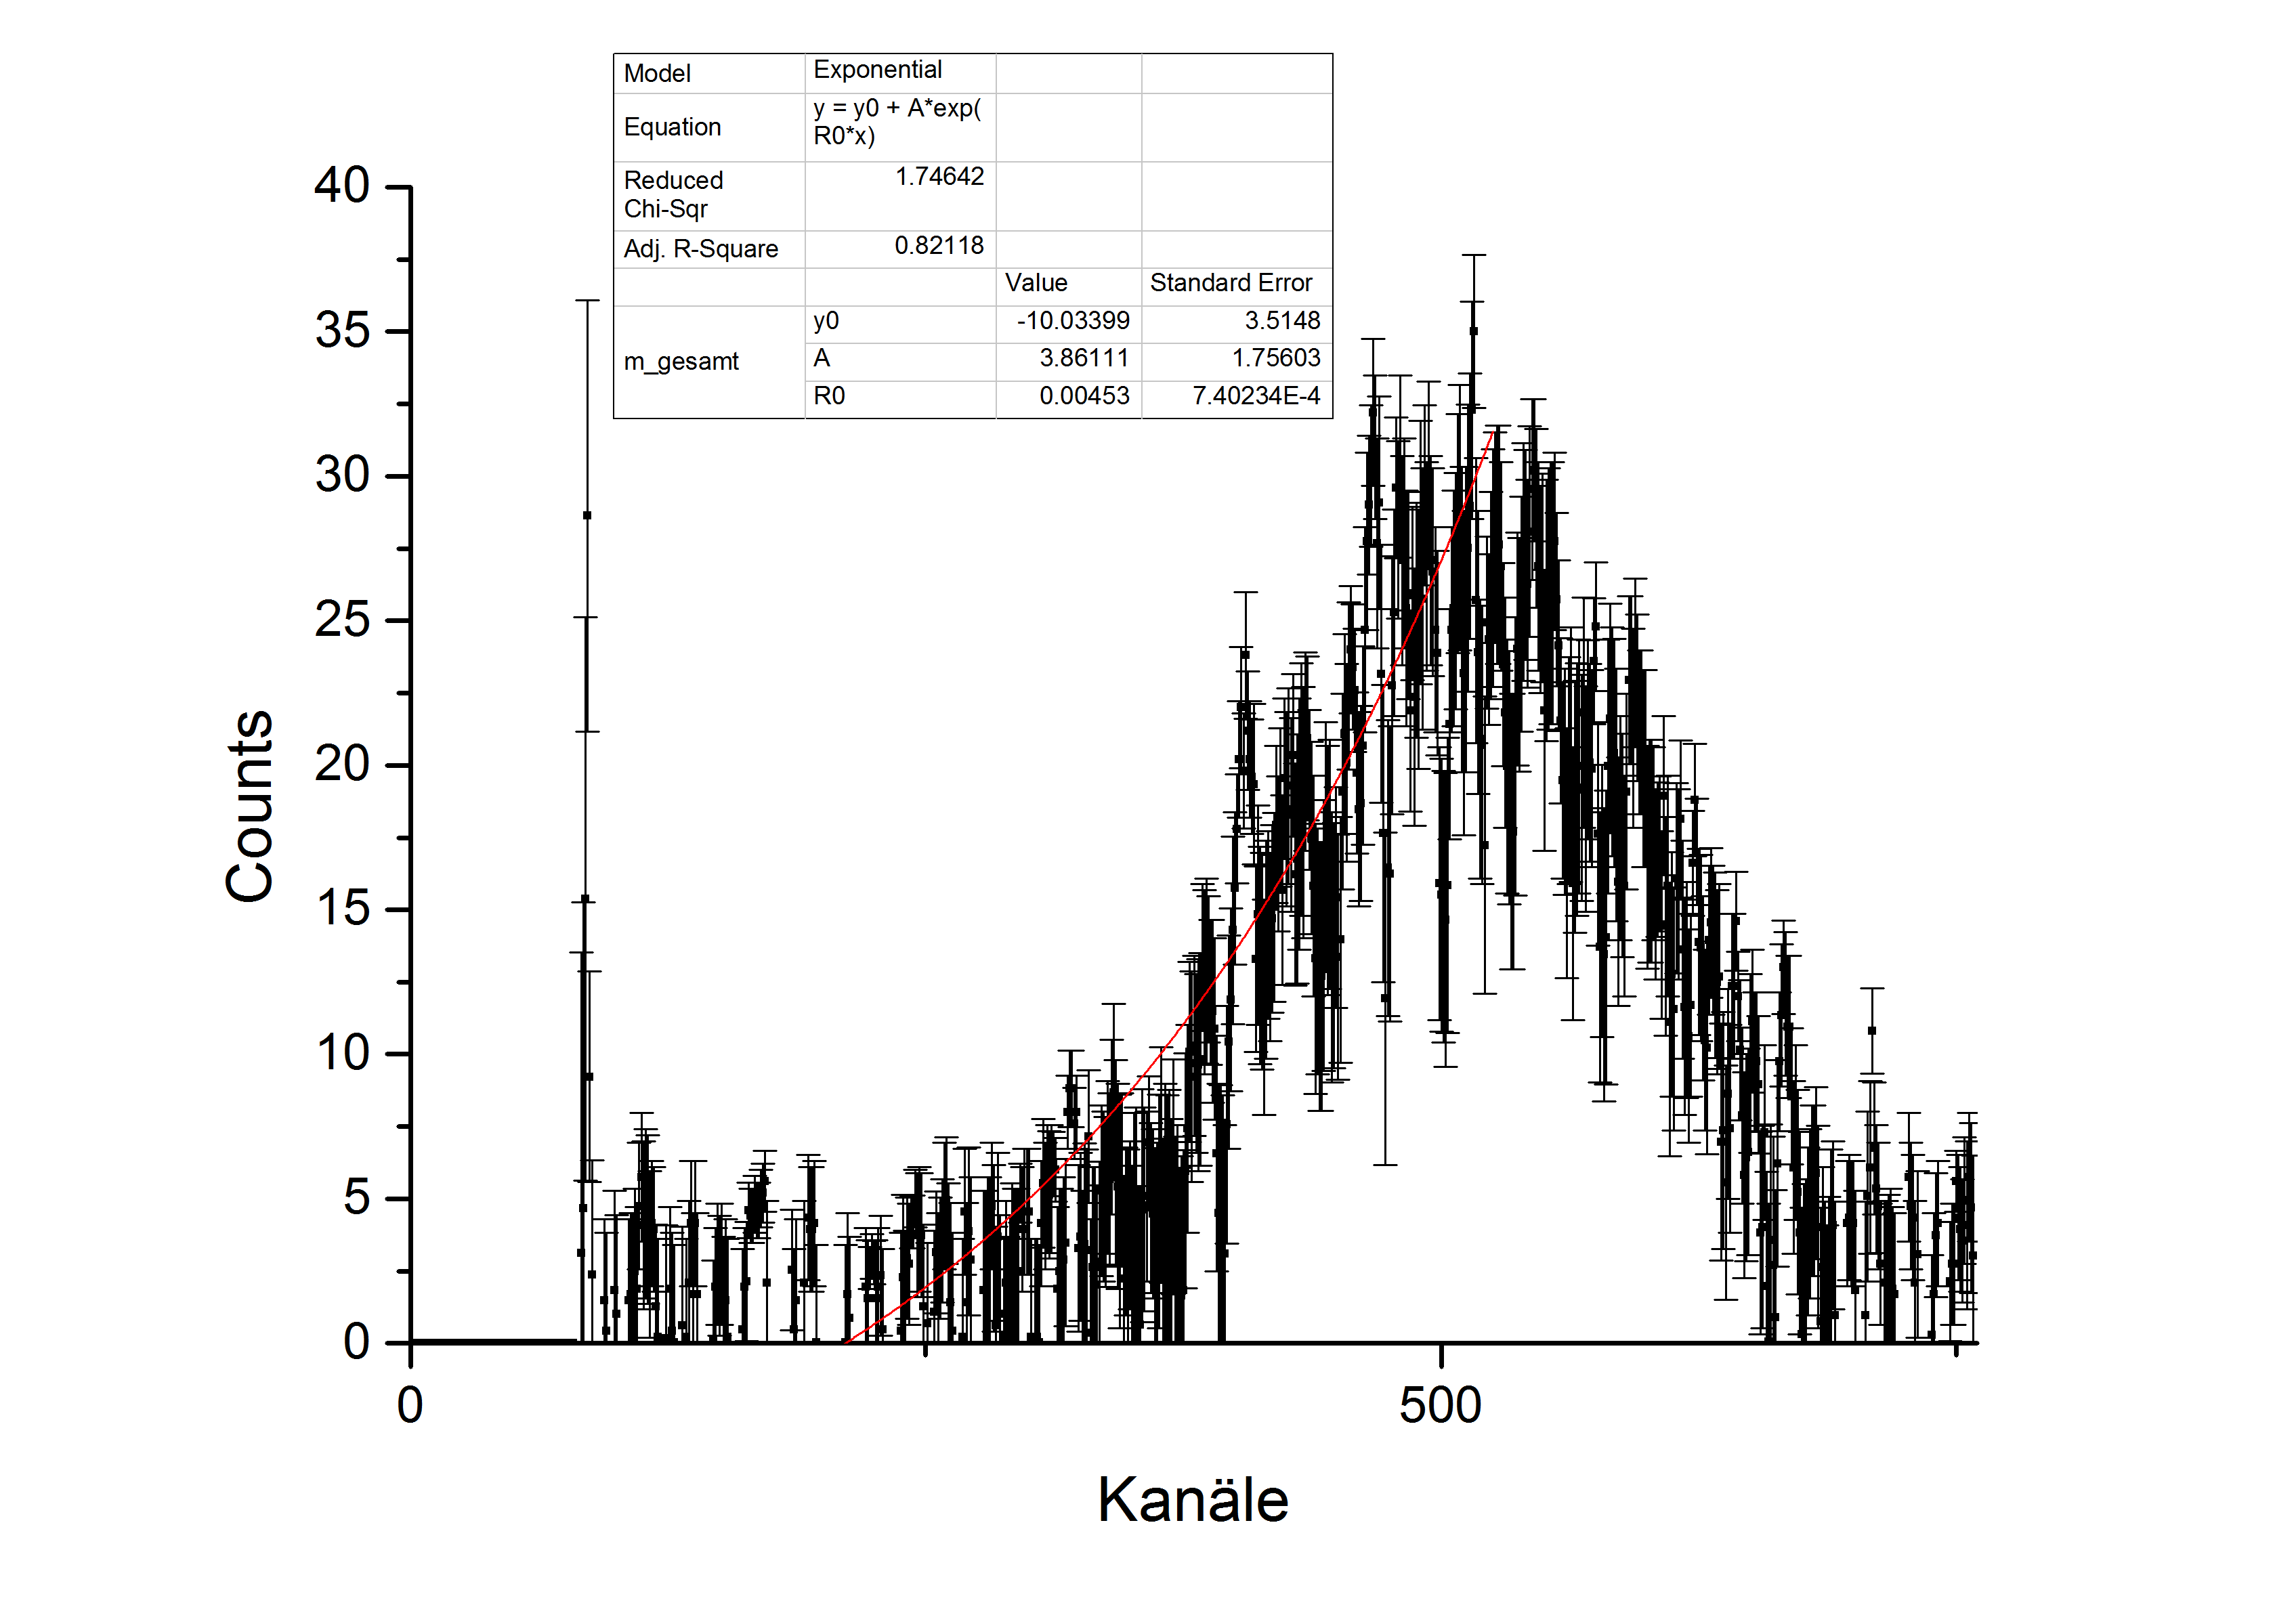
\includegraphics[scale=0.5]{Expfit}
\caption{Spektrum mit Fehlerbalken}
\end{figure}
Wie man sieht, sind die Fehler groß. Dies liegt an der kurzen Messzeit für die zufälligen Koinzidenzen. Der exponentielle Fit ergibt folgenden Wert für den Fitparameter $R_{0}$:\\
$R_{0}=(0,0045\pm 0,0007)\frac{1}{Kanal}$\\
Mit diesem Wert errechnen wir für die mittlere Lebensdauer:\\
$\tau=\frac{b}{R_{0}}=59,3s$\\
Für den Fehler ergibt sich dann: \\
\[s_{\tau}=\tau*\sqrt{\left(\frac{s_{b}}{b}\right)^{2}+\left(\frac{s_{R_{0}}}{R_{0}}\right)^{2}}=9,7ns\]\\
$\Rightarrow \tau=(60\pm10)ns$\\
Für die Halbwertszeit ergibt sich somit:\\
\[\Rightarrow T_{1/2}=\tau*\ln(2)=41,1 ns\]\\
Analog für den Fehler: $s_{T_{1/2}}=s_{\tau}*\ln(2)=6,7 ns$\\
$\Rightarrow T_{1/2}=(41\pm7)ns$\\
Der Literaturwert beträgt $98 ns$ (Quelle: [Ver]). Der von uns bestimmte Wert weicht also stark vom Literaturwert ab. Dies liegt vermutlich vor allem an der Tatsache, dass - wie bereits während der Messung beobachtet - es ein Problem in einem der Geräte gab: Obwohl der Peak, wie von uns mithilfe der Verzögerungen eingestellt, um Kanal 800 entstehen sollte, entstand er etwa bei Kanal 520. Trotz mehrmaliger Neueinstellung und sogar dem Austausch der radioaktiven Quelle in eine andere ${57}^Co$-Quelle konnte dieser Fehler nicht behoben werden. Obwohl es eigentlich nur um die Steigung geht in diesem Versuch, welche bei einem bloßen Verrücken des Peaks unverändert bliebe, scheint es auch zu einer Streckung gekommen sein, was zu einem verminderten Wert für den Fit-Faktor $R_{0}$ führen würde. Dies ist eine mögliche Erklärung für den schlechten Wert, welchen wir erhielten. Es ist uns allerdings nicht möglich, eine sichere Aussage über die Quelle des Fehlers zu treffen, da die getroffenen Einstellungen korrekt waren.\\
\subsubsection{Halbwertszeitbestimmung - Linearer Fit}
Als alternativen Weg haben wir die Halbwertszeit bestimmt, indem wir die y-Achse, welche die Anzahl an Counts anzeigt, logarithmisch skalierten und einen scheinbar linearen Fit durchführten. Die Bereinigung vom Untergrund erfolgt dabei gleich wie zuvor. \\
\begin{figure}[h]
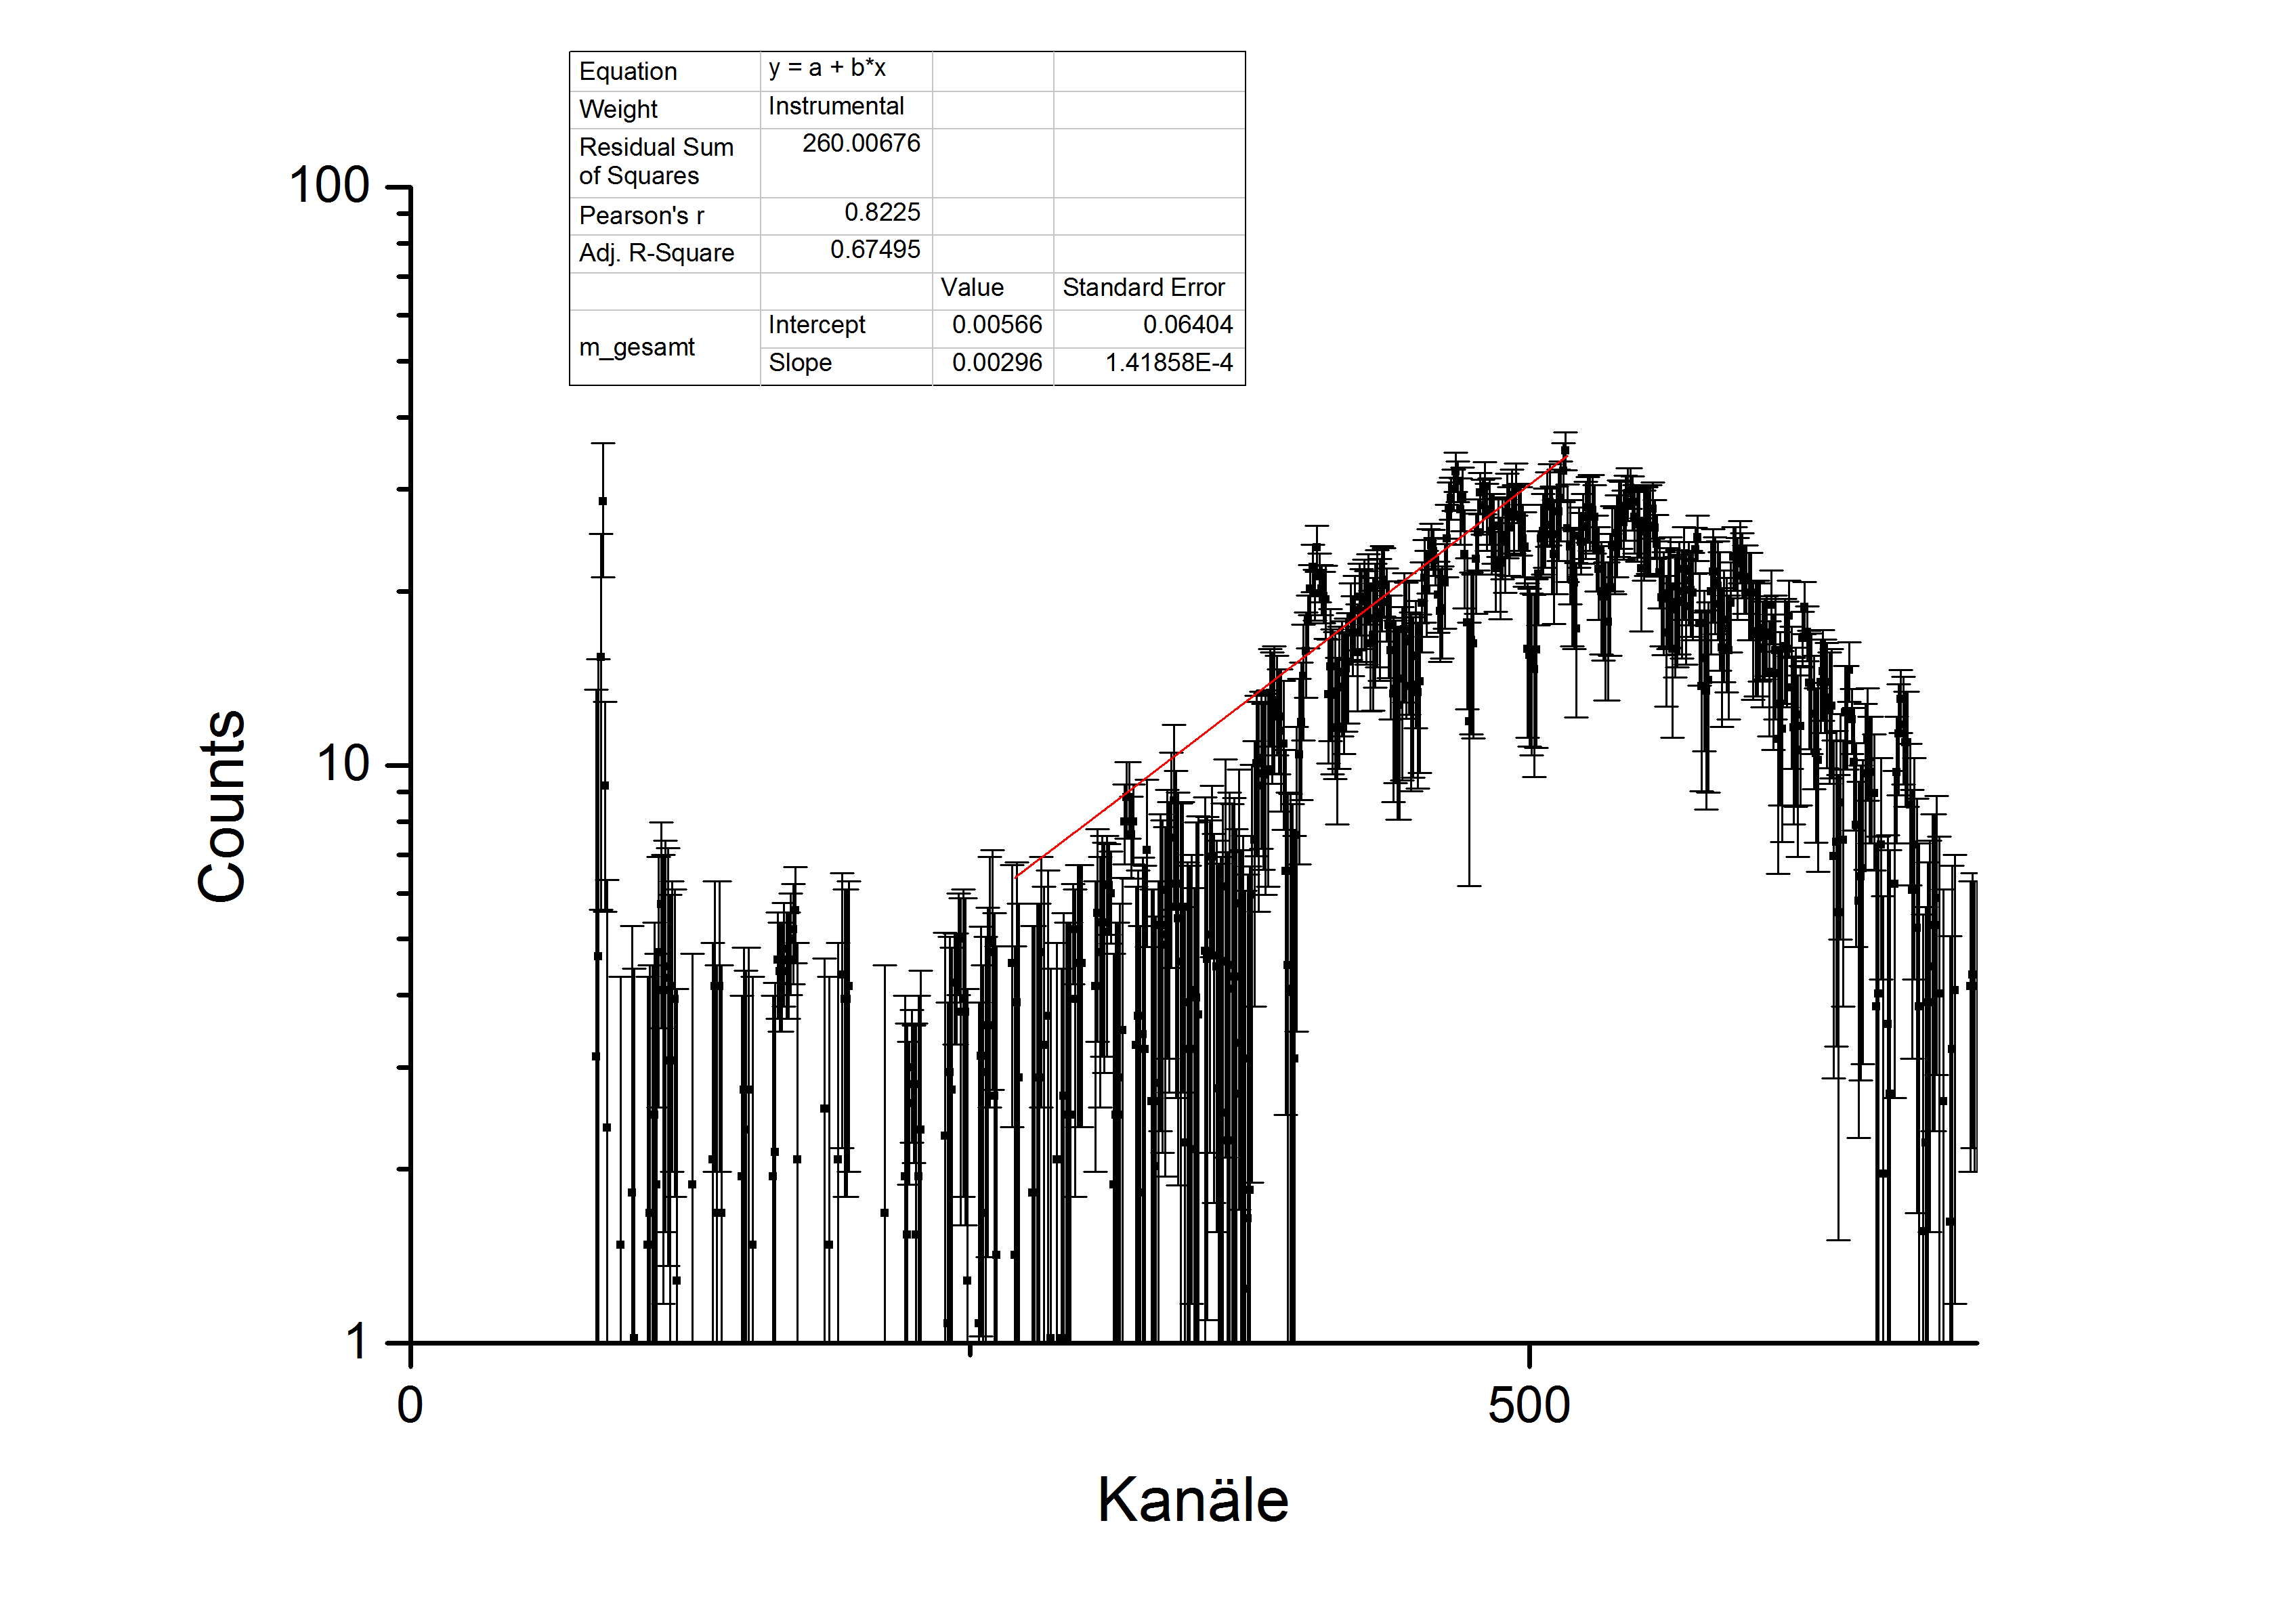
\includegraphics[scale=0.5]{logfit}
\caption{Spektrum mit Fehlerbalken, logarithmisch aufgetragen}
\end{figure}\\
Dabei sind die Fehlerbalken erneut sehr groß, was, wie bereits erwähnt, an der kurzen Messzeit für die zufälligen Koinzidenzen lag. Für die Verbindung zwischen Expontential- und linearem Fit gilt:\\
$y=y_{0}+A*e^{R_{0}*x}$\\
\[\Leftrightarrow \log (y)=\log (y_{0})+\log(A*e^{R_{0}*x})=\log(y_{0})+\log(A)+\log(e^{R_{0}*x})=a+R_{0}*\log(e)*x=a+b*x\]\\
Die Steigung, welche sich für unseren Fit ergibt, ist $b=\frac{(0,00296\pm0,00014)}{Kanal}$, woraus sich für $R_{0}$ folgendes ergibt:\\
$R_{0}=\frac{b}{\log(e)}=\frac{0,0068}{Kanal}$
\[\Rightarrow s_{R_{0}}=\frac{s_{b}}{\log(e)}=\frac{0,0003}{Kanal}\]\\
Damit ergibt sich analog zur exponentiellen Bestimmungsmethode:\\
$\Rightarrow \tau=(39,5\pm1,9)ns$\\
$\Rightarrow T_{1/2}=(27,4\pm1,3)ns$\\
Dieser Wert ist vom Literaturwert von 98 ns (Quelle: [Ver]) noch weiter entfernt, als der mit dem exponentiellen Fit bestimmte. Dies liegt an den sehr großen Fehlern, welche eine große Bandbreite an möglichen linearen Fits zuließ. Die Fehler sind, wie das $\chi^{2}/dof=0,67495$ vermuten lässt (der Wert ist deutlich kleiner als 1), zu groß, um einen sinnvollen Fit erstellen zu können. Dies liegt an der zu kurzen Messdauer für die zufälligen Koinzidenzen, wie bereits diskutiert. Für den exponentiellen Fit gilt $\chi^{2}/dof=0,82118$: Da dieser Wert näher an 1 ist als derjenige für den linearen Fit, können wir davon ausgehen, dass der exponentielle Fit ein realistischeres Ergebnis liefern wird, da die Größe der Fehler weniger ins Gewicht fällt. Dies ist auch tatsächlich der Fall. Ansonsten ist der schlechte Wert, welchen wir durch die Messreihe erhielten wohl ebenso wegen des bereits bei der Durchführung festgestellten Fehlers in der Position des Peaks entstanden.

